%%%%%%%%%%%%%%%%%%%%%%%%%%%%%%%%%%%%%%%%%%%%%%%%%%%%%
% Atenção!!! todo conteudo está organizado modular- %
% mente em seu respectivo arquivo na pasta src.     %
% Favor não encher o main com conteúdo permanente   %
% para facilitar o desenvolvimento do trabalho.     %
%%%%%%%%%%%%%%%%%%%%%%%%%%%%%%%%%%%%%%%%%%%%%%%%%%%%%
\title{Estudo do impacto de ações de re-despacho tendo em conta perturbações em partes da rede elétrica portuguesa}

\documentclass[capchap,sumarioincompleto,a4paper,12pt,ruledheader,normaltoc]{utfprtex}%
\usepackage[utf8]{inputenc}
\usepackage{booktabs}
\usepackage{hyperref}
\usepackage{utfprtexPropostaTCC}
\usepackage{gensymb}
\usepackage{eurosym}
\usepackage{amsmath}
\usepackage[brazil]{babel}
\usepackage[alf,abnt-emphasize=bf,abnt-etal-text=it,bibjustif,abnt-etal-cite=2,abnt-etal-list=0,abnt-full-initials=yes]{abntcite}
\usepackage{graphicx}
\usepackage{float}
\usepackage{amsmath}
\usepackage[table,xcdraw]{xcolor}
\usepackage{multirow}
\usepackage{epstopdf}
\usepackage{lscape}
\DeclareGraphicsExtensions{.eps}
\renewcommand{\floatpagefraction}{0.90}
\renewcommand{\topfraction}{0.95}
\renewcommand{\bottomfraction}{0.95}
\renewcommand{\textfraction}{0.05}
\setlength{\intextsep}{5pt}
\setlength{\textfloatsep}{5pt}
\setlength{\floatsep}{5pt}

\autorA{Callebe Soares Barbosa}
\autorB{Victor Emanuel Soares Barbosa}
\autorC{Carlos Teixeira}
\titulo{Estudo do impacto de ações de re-despacho tendo em conta perturbações em partes da rede elétrica portuguesa} % Título do documento
\local{PORTO}
\data{2017}

%%%%%%%%% Início das definições %%%%%%%%%

\begin{document}

\capa%
\newpage%
\newpage%


% RESUMO:
\begin{Resumo}
Escreva aqui o texto de seu resumo... 
\utfprTeX
\end{Resumo}

\listadefiguras

\listadetabelas

%\listadesiglas

\listadesimbolos

\sumario

%% Capítulos
\chapter{Introdução} 
	\section{Objetivos}
% Simulação
% Caracterização 

\section{Motivações}

\section{Organização do texto}

\chapter{Caracterização da rede elétrica nacional} 
	%------------ SECTION %------------
% Victor
\section{Análise da rede elétrica nacional}
	A produção de energia elétrica em Portugal é aberta ao livre mercado e concorrência, tendo dois regimes legais, a saber \cite{REN-site}:
\begin{itemize}
\item Produção em regime ordinário (PRO): relativo à produção de eletricidade a partir de fontes não renováveis ou em grandes centrais hídricas;
\item Produção em regime especial (PRE): relativo à produção de eletricidade a partir de fontes renováveis ou cogeração.
\end{itemize}

O transporte, ou transmissão, da energia elétrica é realizada através da Rede Nacional de Transporte
%\sigla[Rede Nacional de Transporte]{RNT}% 
, a saber a rede de 150 a 400 kV, através de concessão pelo Estado Português em regime de serviço público e exclusividade à Redes Energéticas Nacionais %\sigla[Redes Energéticas Nacionais]{REN}%
. Tal concessão inclui planeamento, construção, operação e manutenção da RNT \cite{REN-site}.

A rede de distribuição é efetivada através da exploração da Rede Nacional de Distribuição %\sigla[Rede Nacional de Distribuição]{RND}%
. A rede de baixa tensão é operada através de contratos estabelecidos entre os municípios e as distribuidoras \cite{REN-site}.

Em relação ao consumo, no Portugal Continental há 6,1 milhões de consumidores em maioria na baixa tensão, 23 500 na média tensão, 350 na alta tensão e muito alta tensão, até 400 kV. O consumidor é livre para escolher o seu comercializador de energia elétrica \cite{REN-site}.

O Sistema Elétrico Nacional %\sigla[Sistema Elétrico Nacional]{SEN}
, ilustrado de forma simplificada na Figura \ref{fig:Organizacao_SEP_PT}, é composto pela parte da produção: PRO, PRE e importação; pela parte do transporte: RNT; pela parte de comercialização: Comercializador Liberalizado e Comercializador de Último Recurso %\sigla[Comercializador de Último Recurso]{CUR}%
; e por fim, pela parcela da distribuição: clientes do mercado liberalizado e do CUR. Os comercializadores liberalizados e de último recurso estão enquadrados no Mercado Organizado. A Entidade Reguladora dos Serviços Energéticos %\sigla[Entidade Reguladora dos Serviços Energéticos]{ERSE}%
é quem estabelece as tarifas pagas pelos comercializadores para acenderem à RNT e RND. Todo esse sistema está sob o enquadramento legislativo e regulamentar da Direção Geral de Energia e Geologia %\sigla[Direção Geral de Energia e Geologia]{DGGE}%
\cite{gil2010analise}.

\begin{figure}[H]
	\centering
	\captionsetup{width=\textwidth, font=footnotesize, textfont=bf}	
	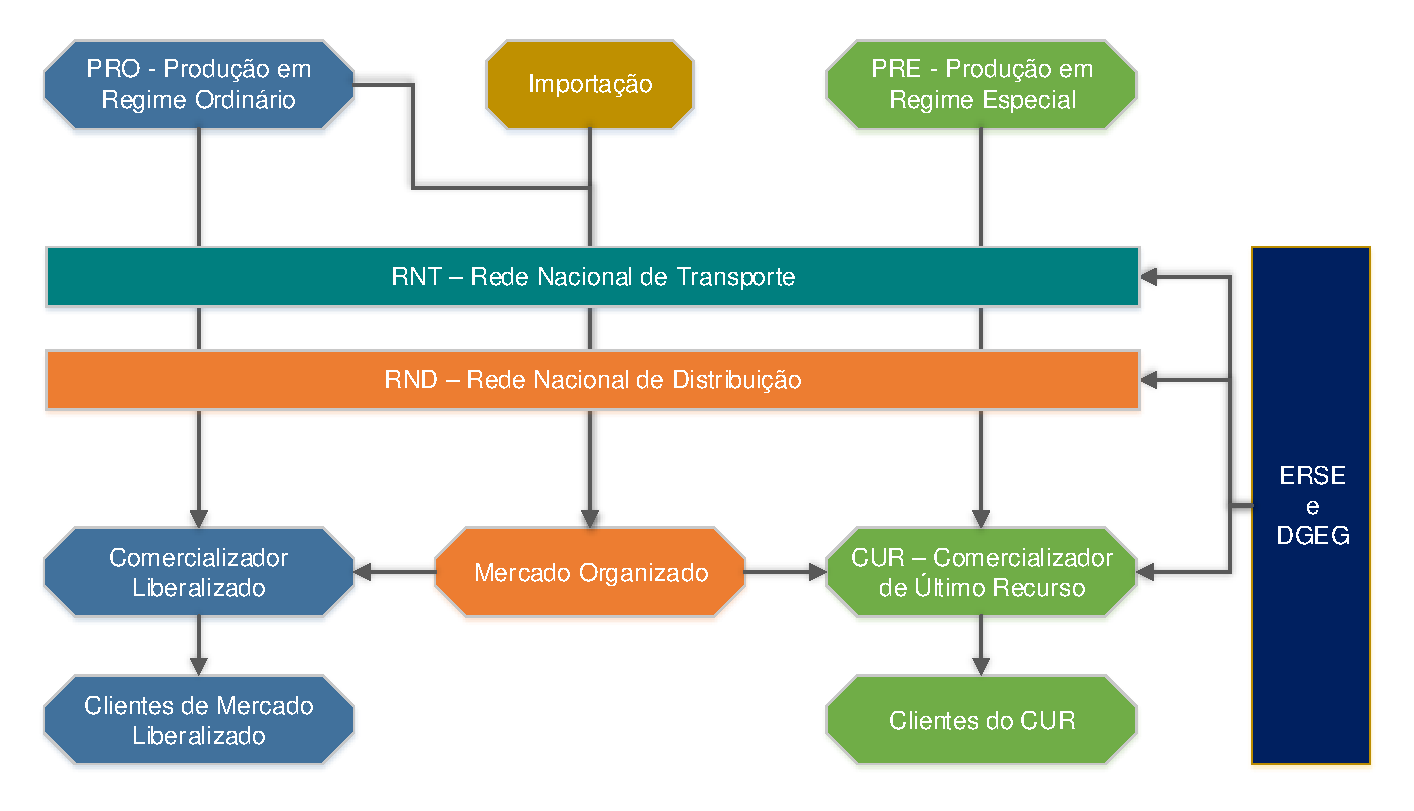
\includegraphics[width=\textwidth]{img/Organizacao_SEP_PT.pdf}
	\caption{Esquema simplificado da Organização do Sistema Elétrico Nacional.}
	\vspace{-3.5mm}
	\caption*{Fonte: \cite{gil2010analise}}
	\label{fig:Organizacao_SEP_PT}
\end{figure}


%------------ SECTION %------------
% Carlos
\section{Caracterização das centrais}
	\input{src/Caracterizacao_rede/Caracterizacao_das_centrais.tex}

% Localização; 
% potência Instalada;
% Especificações

%----------- SECTION %------------
% Carlos
\section{Caracterização da RNT}
	\input{src/Caracterizacao_rede/Caracterizacao_da_RNT.tex} 

% Capacidade; 
% especificações

%------------ SECTION %------------
% Callebe
\section{Perfil de produção nacional}
	Segunda a \citeonline[p.~5]{e2p}, desde 2000 as fontes renováveis apresentaram um crescimento continuo na matriz energética portuguesa, sobre tudo a geração eólica. Este franco crescimento foi proveniente de uma política europeia e nacional que tem como objetivo a melhoria da segurança de abastecimento, redução da dependência energética e redução dos impactos ambientais do sistema elétrico.  

Como resultado da política energética portuguesa, em 2016  57\% da produção de energia elétrica em Portugal se deu através de fontes renováveis. Face ao ano anterior as fontes renováveis aumentaram 10\% na participação da produção \cite[p.~8]{REN}. O aumento da produção renovável e 2016 deve-se, em parte, da entrada da central hidroelétrica de Frades II, equipada com 780 MW, e do crescimento em 236 MW de potência instalada em parques eólicos portugueses. Seguindo assim uma tendência de crescimento desde 2014, o que pode ser verificada através das estatísticas diária disponibilizadas pela \citeonline{REN-site}.  Em 2016 a geração hidráulica representou 28\% da produção nacional, enquanto a geração eólica representou 22\%, a biomassa representou 5\% e a solar contribuiu com 1\%.

Um fato importante sobre a geração renovável em 2016 é que devido a sua grande participação na produção de energia houve uma redução no preço médio do MWh no mercado ibérico de eletricidade, valor este que esteve situado em 39,4 \euro/MWh \cite[p.~4]{apren}. Comparado ao ano de 2015, quando o custo médio esteve em 50,4 \euro/MWh e a contribuição das renováveis para a matriz energética foi de 48 \%, nota-se uma relação entre o custo \euro/MWh e a  produção renovável. A Figura \ref{fig:CorrelacaoPrecoMercadoProducaoRenovavel} deixa mais explicita esta relação entre o anos de 2015 e 2016.

\begin{figure}[H]
	\centering
	\captionsetup{width=0.85\textwidth, font=footnotesize, textfont=bf}
	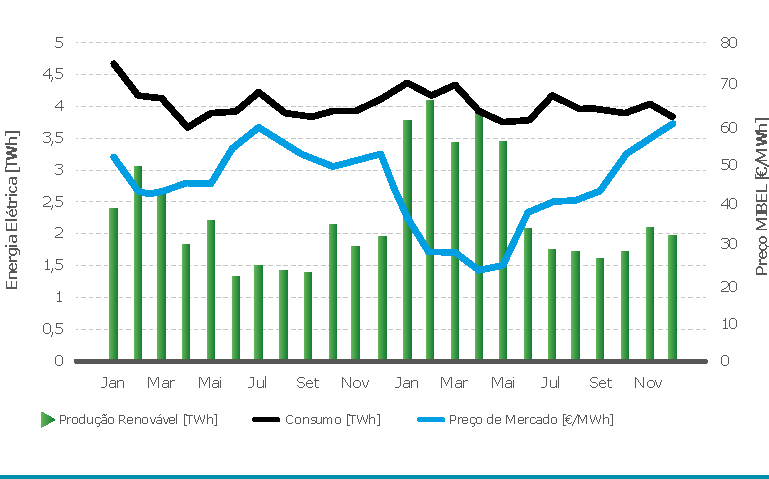
\includegraphics[width=0.8\linewidth]{img/CorrelacaoPrecoMercadoProducaoRenovavel.pdf}
	\caption{Correlação entre o Preço de Mercado e a Produção Renovável (2015-16) }
	\vspace{-3.5mm}
	\caption*{Fonte: \citeonline[p.~10]{apren}}
	\label{fig:CorrelacaoPrecoMercadoProducaoRenovavel}
\end{figure}

Já pelo lado das fontes não renováveis a geração por termoelétricas a carvão e a gás natural ambas representaram, em 2016, 21\% da produção. Face ao ano anterior a produção a carvão sofreu uma queda de 14\%, já a produção a gás natural cresceu 18\% \cite[p.~8]{REN}. Os dados a produção nacional em 2016 estão dispostas Gráfico \ref{fig:ReparticaoDaProducao}, e para fins de comparação está a Tabela \ref{tab:producao20152016}.

\begin{figure}[H]
	\centering
	\captionsetup{width=0.7\textwidth, font=footnotesize, textfont=bf}
	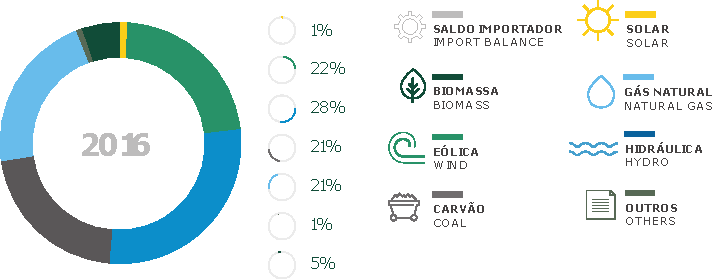
\includegraphics[width=0.7\linewidth]{img/ReparticaoDaProducao2016.pdf}
	\caption{Repartição da Produção}
	\vspace{-3.5mm}
	\caption*{Fonte: \citeonline[p.~8]{REN}}
	\label{fig:ReparticaoDaProducao}
\end{figure}

\begin{table}[H]
	\centering
	\captionsetup{width=0.74\textwidth, font=footnotesize, textfont=bf}
    \begin{tabular}{|l|c|c|c|}
    \rowcolor[HTML]{000000}
    {\color[HTML]{FFFFFF} Geração} & {\color[HTML]{FFFFFF} 2015} & {\color[HTML]{FFFFFF} 2016}   & {\color[HTML]{FFFFFF} Variação(\%) }  \\
    Hídrica                 & 8.453  & 15.413 & 82           \\
    Eólica                  & 11.334 & 12.188 & 8            \\
    Biomassa                & 2.618  & 2.687  & 3            \\
    Solar                   & 760    &  781   & 3            \\
    Carvão                  & 13.677 & 11.698 & -14          \\
    Gás Natural             & 9.807  & 11.571 & 18           \\
    Produção por Bombagem   & 1.160  & 1.217  & 5            \\
    Saldo Importador        & 2.266  & -5.085 & -            \\ \hline
    Produção Não Renovável  & 23.840 & 23.587 & -1           \\ \hline
    Produção Renovável      & 23.165 & 31.069 & 34           \\ \hline
    Produção Total          & 48.165 & 55.873 & 16           \\ \hline
    \end{tabular}
    \caption{Produção Nacional 2015/2016}
    \vspace{-3.5mm}
	\caption*{Fonte: \citeonline[p.~10]{REN}}
    \label{tab:producao20152016}
\end{table}


%------------ SECTION %------------
% Callebe
\section{Perfil de Consumo Nacional}
	Em relação ao consumo nacional Portugal vem apresentando um crescimento continuo desde 2012, e se consolida em 2016 com um total de  49,3 TWh, um consumo menor apenas 5,6\% do máximo histórico registrado em 2010. Tal crescimento no consumo tem relação direta com o crescimento social e económico do pais, e indica uma tendência para os próximos anos\cite[p.~6]{REN}. 

O gráfico da Figura \ref{fig:ConsumoMax} apresenta a relação dos máximos de consumo e produção registrados desde 2012. Este gráfico torna claro a evolução dos picos de produção sobre os máximos de consumo ao longo dos anos. A relação entre picos de produção e consumo representam uma margem que assegura atendimento da carga mesmo nos dias de maior pico.

\begin{figure}[H]
	\centering
	\captionsetup{width=0.7\textwidth, font=footnotesize, textfont=bf}	
	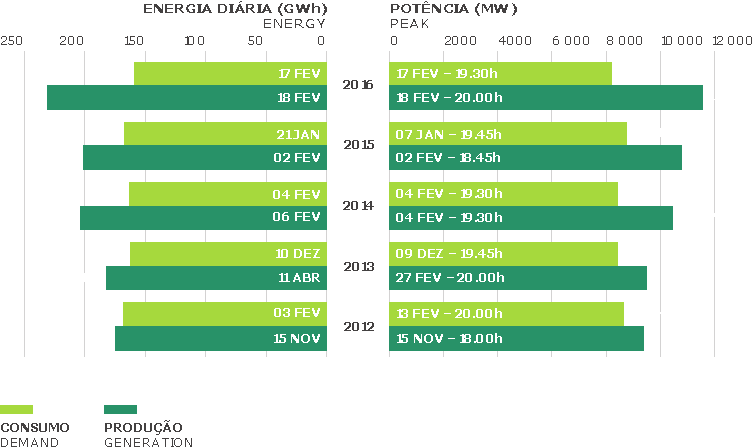
\includegraphics[width=0.7\linewidth]{img/ConsumoEProducaoMaximosAnuais.pdf}
	\caption{Consumo e Produção Máximos Anuais}
	\vspace{-3.5mm}
	\caption*{Fonte: \citeonline{REN}}
	\label{fig:ConsumoMax}
\end{figure}

Em 2016 o dia de maior pico no consumo ocorreu no dia 17 de fevereiro, já em 2015 o dia de maior pico no consumo foi registrado no dia 7 de janeiro. Mas apenas em  2016, mesmo no horário de pico todo o consumo foi atendido pela geração nacional, ou seja não houve saldo importador. Como pode ser visto na Figura \ref{fig:ConsumoDiaDePontaAnual} \cite{apren}.

\begin{figure}[H]
	\centering
	\captionsetup{width=0.7\textwidth, font=footnotesize, textfont=bf}	
	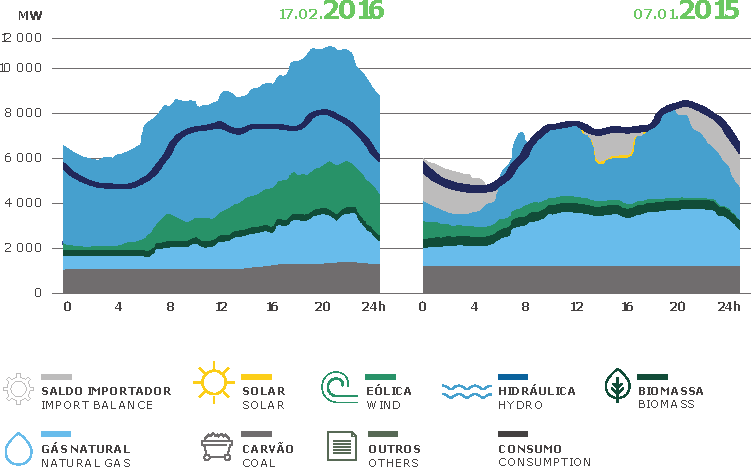
\includegraphics[width=0.7\linewidth]{img/ConsumoDiaDePontaAnual.pdf}
	\caption{Diagrama de Consumo no Dia de Ponta Anual}
	\vspace{-3.5mm}
	\caption*{Fonte: \citeonline{REN}}
	\label{fig:ConsumoDiaDePontaAnual}
\end{figure}

Em 2016 houve um total de  1130 horas em que a eletricidade renovável por si só, foi suficiente para suprir as necessidades elétricas de Portugal. Ainda neste ano, entre as 6:45h do dia 7 e 17:45h do dia 11 de maio, foi registrado um período de 107 horas consecutivas em que a produção renovável excedeu o consumo elétrico \cite{apren}. Estes fato que demonstra que mesmo com o aumento do consumo, a geração renovável e supera o consumo em vários períodos relevantes. 

Segundo a \citeonline{apren} em 2016 houve um importante marco do saldo exportador de 5,1 TWh, que constitui uma inversão na tendência de importação apresentada nos últimos 15 anos. O gráfico da Figura \ref{fig:SatisfacaoDoConsumo} trás um comparativo da satisfação do consumo anual entre 2007 e 2016. 

\vspace{5.5mm}

\begin{figure}[H]
	\centering
	\captionsetup{width=0.7\textwidth, font=footnotesize, textfont=bf}	
	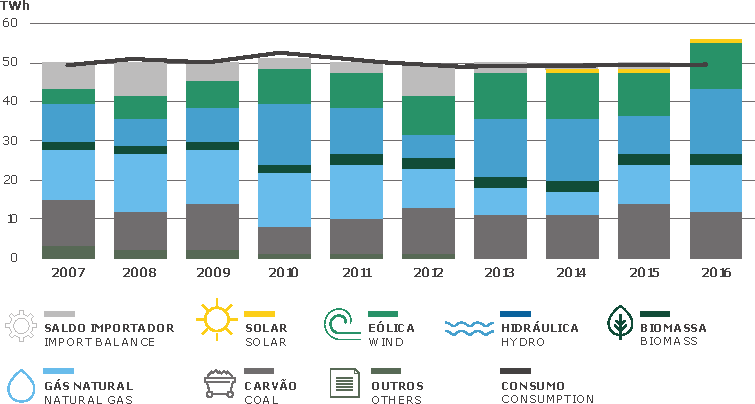
\includegraphics[width=0.7\linewidth]{img/SatisfacaoDoConsumo.pdf}
	\caption{Satisfação do Consumo}
	\vspace{-3.5mm}
	\caption*{Fonte: \citeonline[p.~10]{REN}}
	\label{fig:SatisfacaoDoConsumo}
\end{figure}






\chapter{Cenários Proposto}
	% ---------- CENÁRIO 1 ----------
\section{Cenário 1} % Callebe
	\subsection{Anterior à modificação}

A região escolhida para o cenário 1 foi a interligação entre a subestação de Bouca e Zezere, na região central de Portugal como pode ser visto na Figura \ref{fig:caso1}. A mudança no cenário atual é a retirada de uma das duas linha que interligam o barramento da subestação de Bouca com o barramento de 145 kV de Zezere, o qual pode ser vista na Figura \ref{fig:caso1After}.

\vspace{3.3mm}

\begin{figure}[H]
	\centering
	\captionsetup{width=1\textwidth, font=footnotesize, textfont=bf}	
	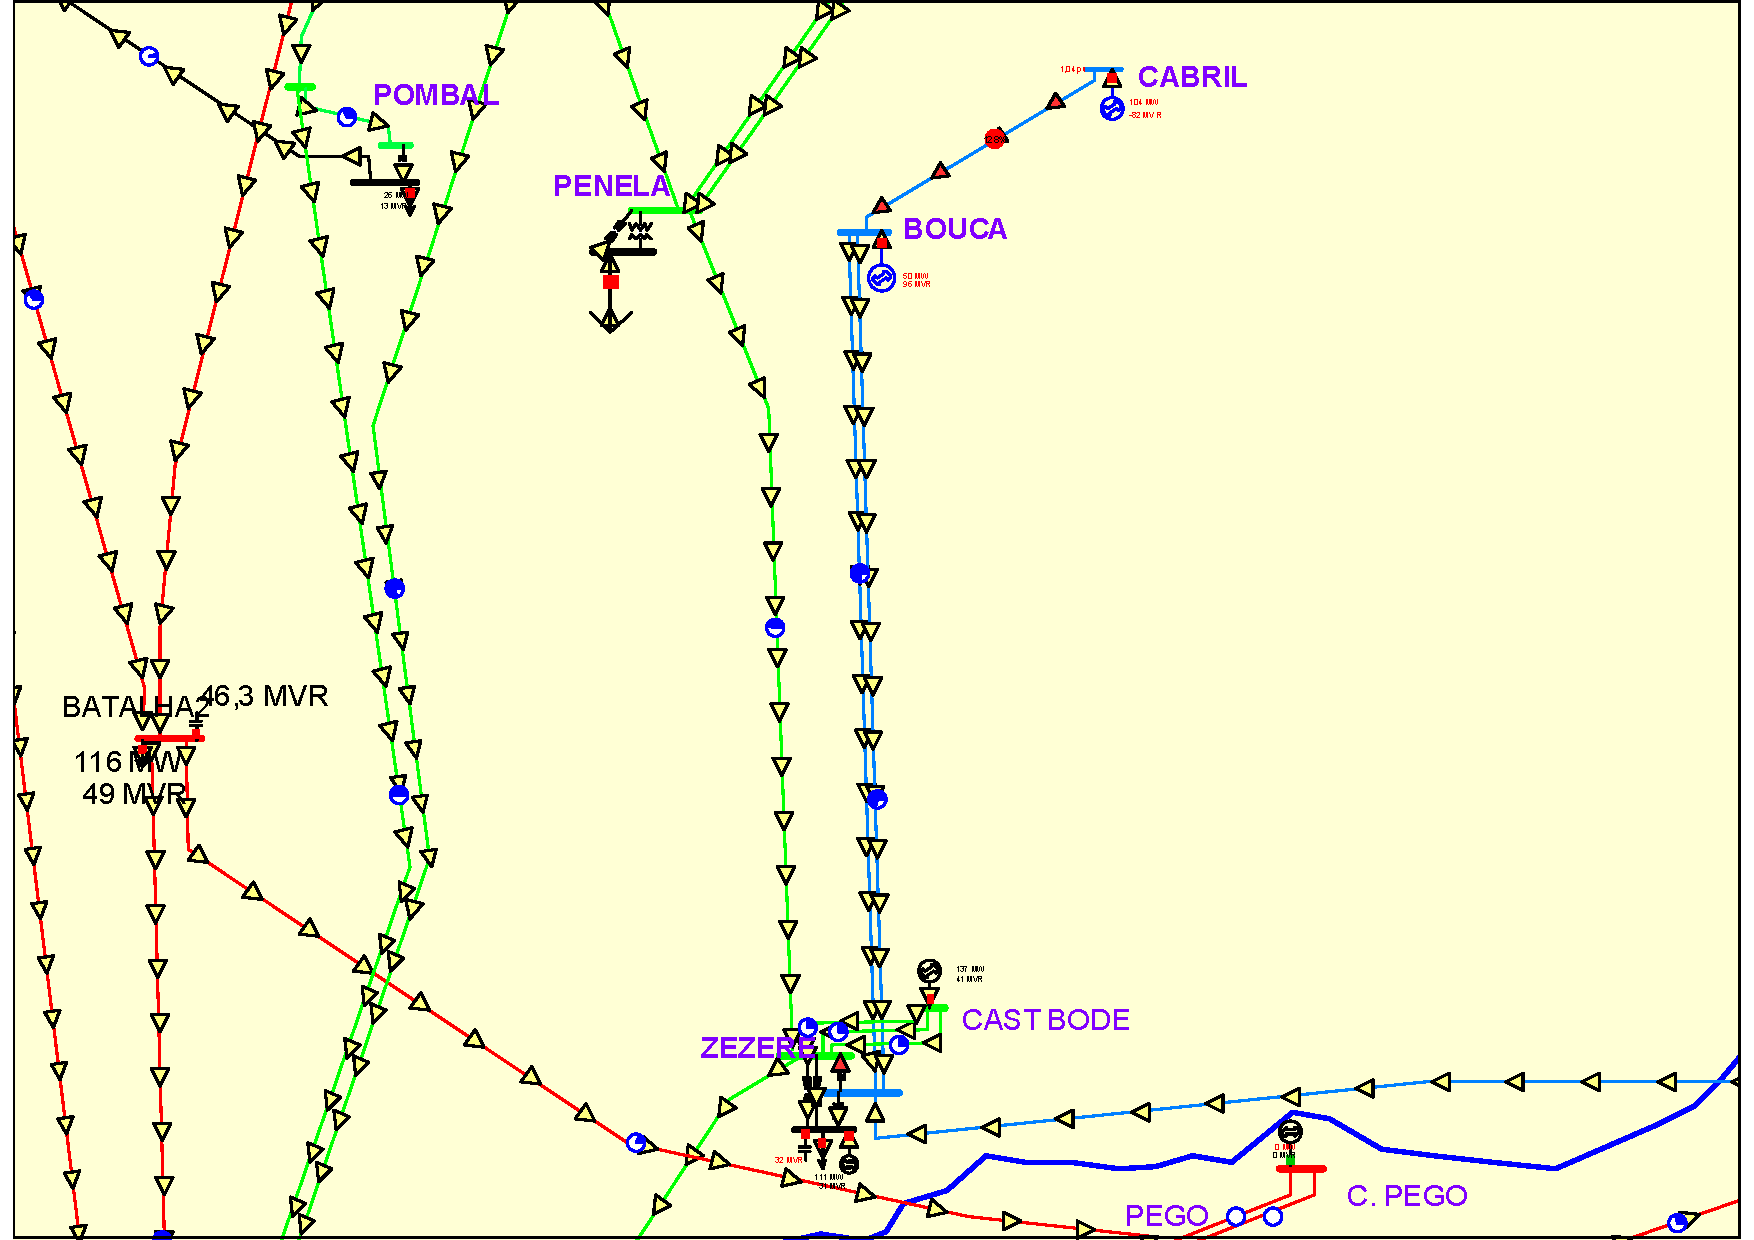
\includegraphics[width=1\linewidth]{img/caso1.pdf}
	\caption{Cenário 1, anterior à modificação}
	\vspace{-3.5mm}
	\caption*{Fonte: Caso Simulado no \textit{PowerWorld\textsuperscript{\textregistered} Simulator}}
	\label{fig:caso1}
\end{figure}

A subestação de Bouca se interliga apenas com o barramento de 145 kV de Zezere e com o barramento de Cabril, o qual possui uma unidade geradora de 104 MW. Existe apenas uma linha de Bouca a Zezere o qual apresenta uma sobrecarga 128\% no transito de potência no sentido Cabril Bouca. A interligação entre bouca e Zezere é feita por duas linhas que apresentam respectivamente  72,5\% e 72,6\% de carregamento.

\begin{figure}[H]
	\centering
	\captionsetup{width=1\textwidth, font=footnotesize, textfont=bf}	
	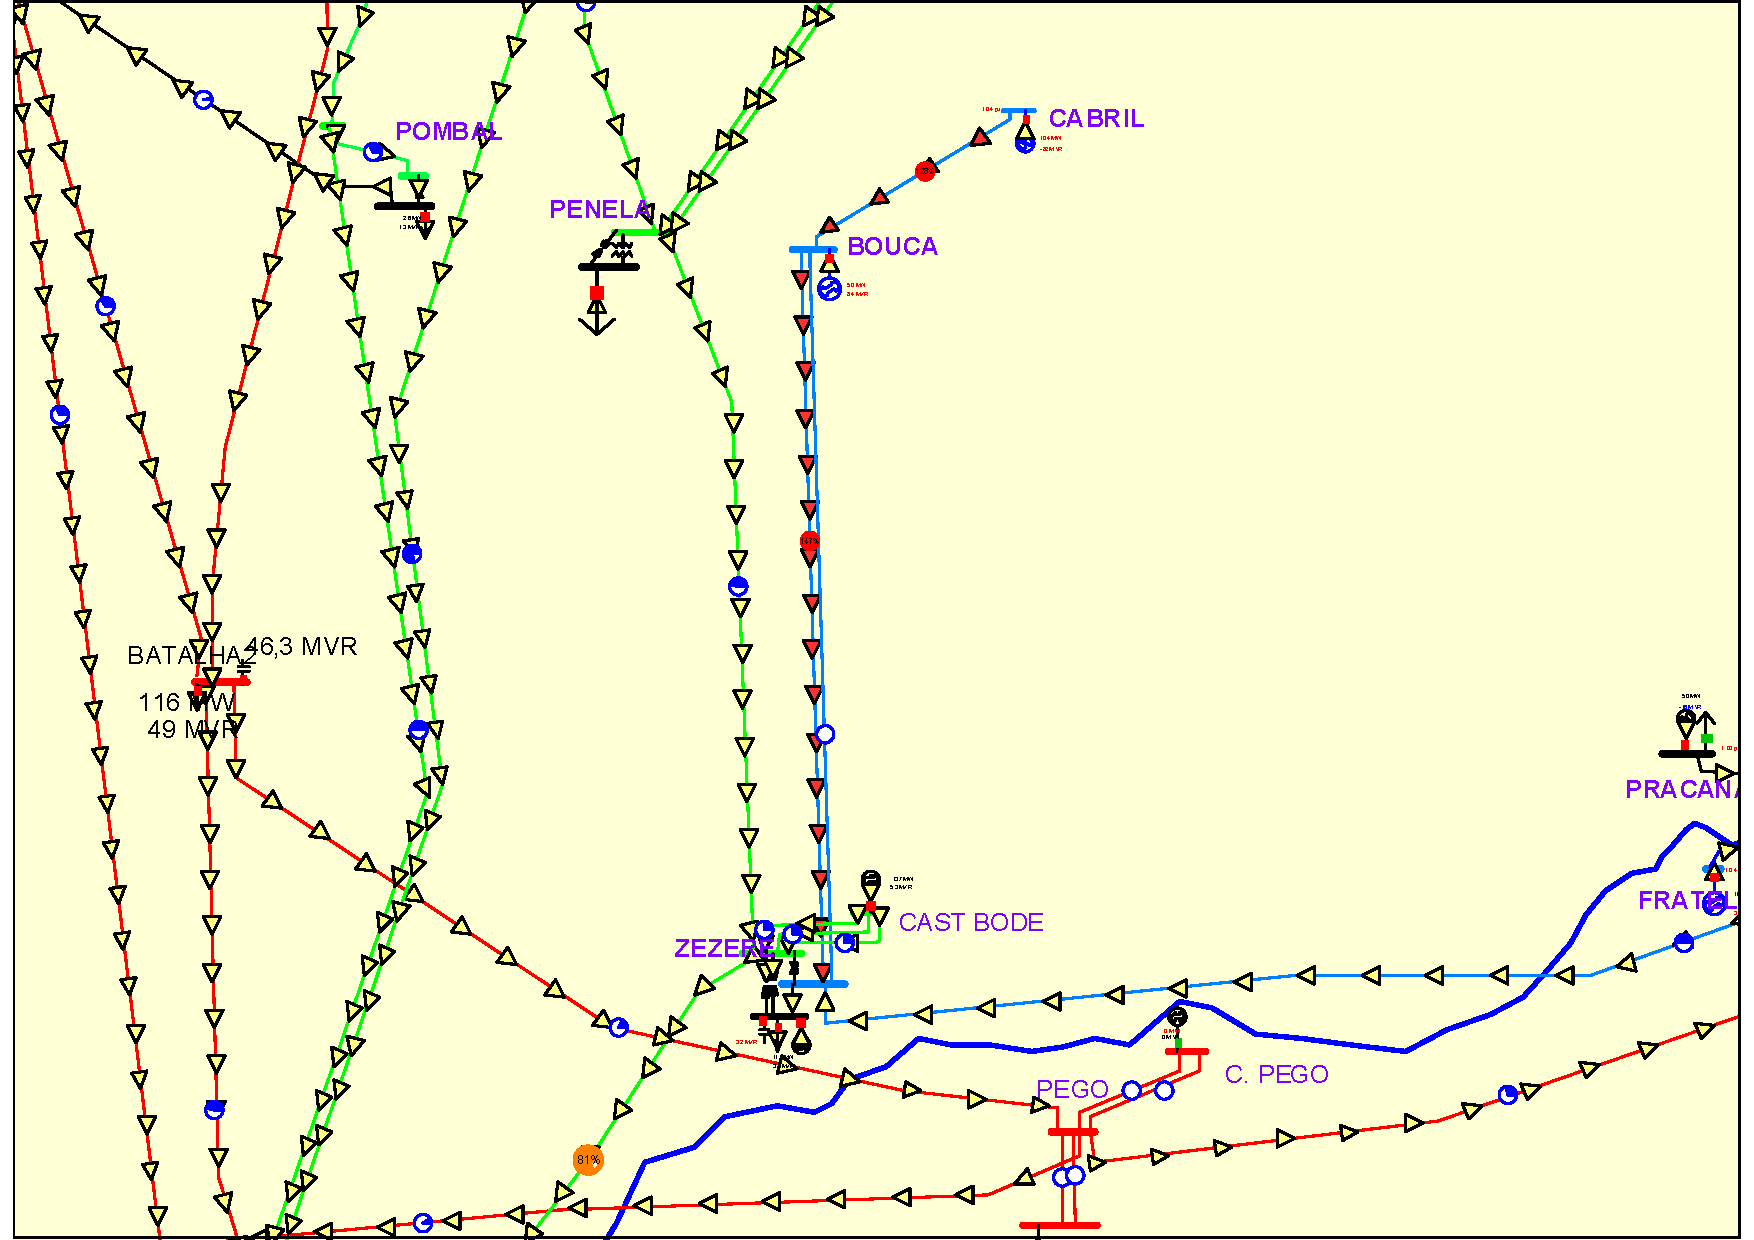
\includegraphics[width=1\linewidth]{img/caso1After.pdf}
	\caption{Cenário 1, após à modificação}
	\vspace{-3.5mm}
	\caption*{Fonte: Caso Simulado no \textit{PowerWorld\textsuperscript{\textregistered} Simulator}}
	\label{fig:caso1After}
\end{figure}

A subestação de Zezere possui 3 barramentos; o primeiro de 145 kV que interligam a Bouca e Falaguei, o segundo que 230 kV que interligam Santarem, Penela e Cast Bode. O terceiro barramento de 63 kV é onde está conectado uma carga de 111M e um gerador de 22,1 MW. Os dados globais do sistema antes das alterações propostas estão dispostas na tabela \ref{tab:DadosGeraisIniciais}. Já os dados locais relativos as barras próximas a modificação proposta, estão dispostos na Tabela \ref{tab:DadosLocaisIniciais}.

\begin{table}[H]
\centering
	\captionsetup{width=0.4\textwidth, font=footnotesize, textfont=bf}
    \begin{tabular}{|
  >{\columncolor[HTML]{333333}}l |c|c|l}
  \cline{1-3}
  {\color[HTML]{FFFFFF} }        & \cellcolor[HTML]{333333}{\color[HTML]{FFFFFF} MW} & \cellcolor[HTML]{333333}{\color[HTML]{FFFFFF} MVAr} &  \\ \cline{1-3}
  {\color[HTML]{FFFFFF} Perdas}  & 229,50                                            & -376,75  &  \\ \cline{1-3}
  {\color[HTML]{FFFFFF} Geração} & 6794,0                                             & -306,1  &  \\ \cline{1-3}
  {\color[HTML]{FFFFFF} Cargas}  & 6564,5                                            & 1814,2 &  \\ \cline{1-3}
  \end{tabular}
  \caption{Dados globais iniciais}
  \vspace{-3.5mm}
	\caption*{Fonte: Autoria Própria}
  \label{tab:DadosGeraisIniciais}
\end{table}

\begin{table}[H]
\centering
\captionsetup{width=0.4\textwidth, font=footnotesize, textfont=bf}
\begin{tabular}{lcc}
\multicolumn{3}{c}{\cellcolor[HTML]{333333}{\color[HTML]{FFFFFF} Carregamento das Linhas}} \\
\multicolumn{1}{c}{}          & \multicolumn{2}{c}{Carregamento (\%)}                \\
Cabril                              & \multicolumn{1}{l}{Bouca}            & 128,5         \\
Bouca                               & \multicolumn{1}{l}{Zezere}           & 73,4          \\
Falaguei                            & \multicolumn{1}{l}{Zezere}           & 52,6          \\
Panela                              & \multicolumn{1}{l}{Zezere}           & 47,1          \\
Zezere                              & \multicolumn{1}{l}{Santarem}         & 81,5          \\
Cast Bode                           & \multicolumn{1}{l}{Zezere}           & 25            \\
\multicolumn{3}{c}{\cellcolor[HTML]{333333}{\color[HTML]{FFFFFF} Tensão nas Barras}}       \\
\multicolumn{1}{c}{}           & Módulo                               & Ângulo        \\
Cabril                              & 1,04                                 & 30,889        \\
Bouca                               & 1,05                                 & 29,566        \\
Zezere                              & 1,0399                               & 22,006        \\
Falaguei                            & 1,03                                 & 30,919        \\
Panela                              & 1,0473                               & 26,098        \\
Santarem                            & 1,0269                               & 14,32         \\
Cast Bode                           & 1,04                                 & 22,019        \\
\multicolumn{3}{c}{\cellcolor[HTML]{333333}{\color[HTML]{FFFFFF} Geradores}}               \\
\multicolumn{1}{c}{}         & MW                                   & Mvar          \\
Cabril                              & 104,2                                & -82,29        \\
Bouca                               & 49,6                                 & 96,14         \\
Zezere                              & 22,1                                 & -23,24        \\
Cast Bode                           & 137,2                                & 41,46         \\
Falaguei                            & 148                                  & 65,76        
\end{tabular}
\caption{Dados Locais Iniciais}
  \vspace{-3.5mm}
	\caption*{Fonte: Autoria Própria}
  \label{tab:DadosLocaisIniciais}
\end{table}


\subsection{Análise do impacto da modificação}


\subsubsection{Análise global}

\begin{figure}[H]
	\centering
	\captionsetup{width=\textwidth, font=footnotesize, textfont=bf}	
	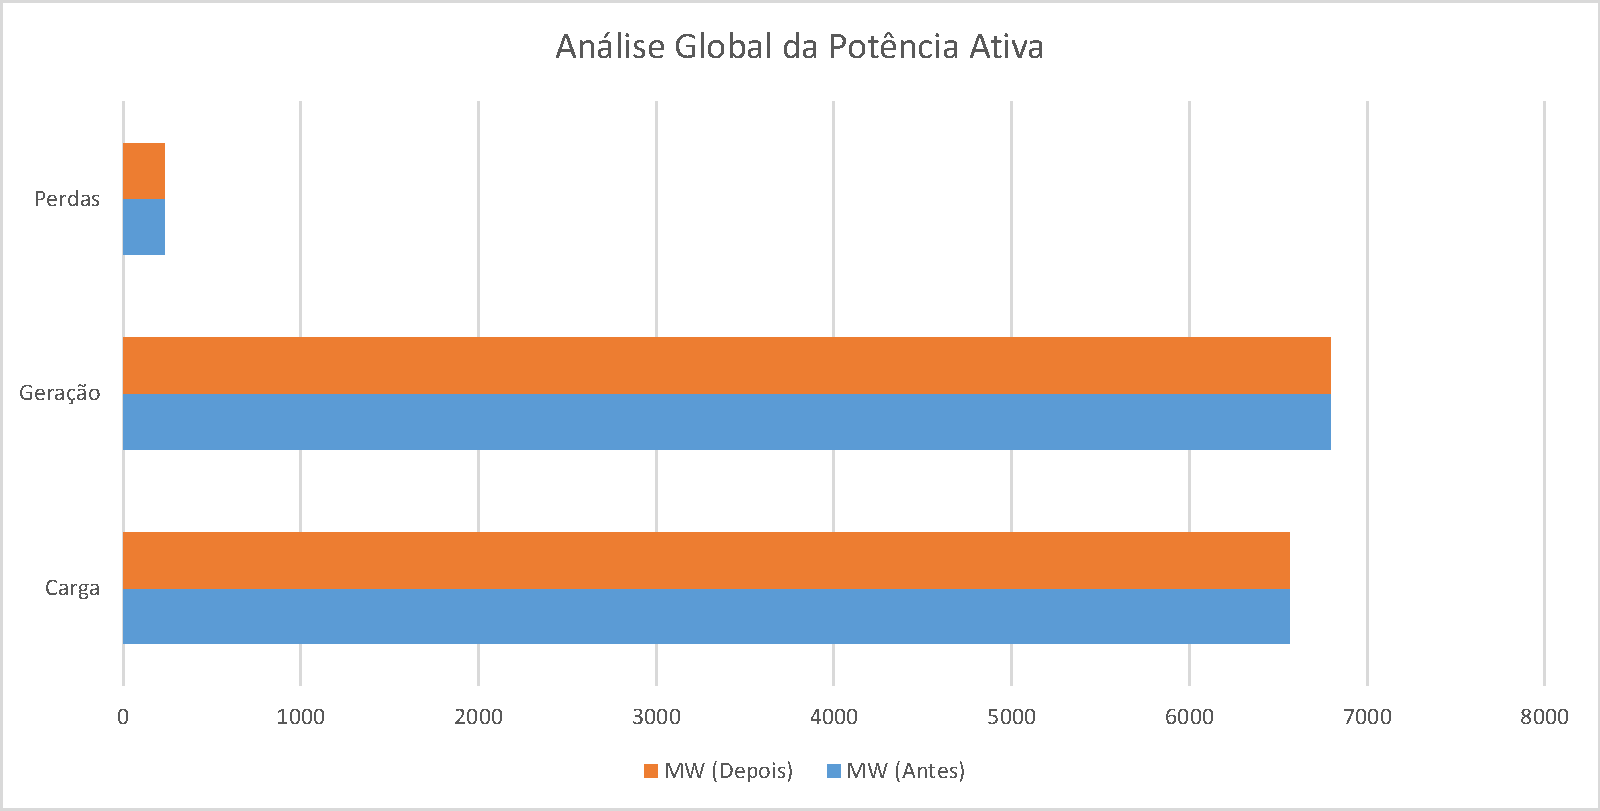
\includegraphics[width=\linewidth]{img/global_MW_caso1.pdf}
	\caption{Análise ativa global antes e após o cenário 1}
	\vspace{-3.5mm}
	\caption*{Fonte: autoria própria}
	\label{fig:global_MW_caso1}
\end{figure}

\begin{figure}[H]
	\centering
	\captionsetup{width=\textwidth, font=footnotesize, textfont=bf}	
	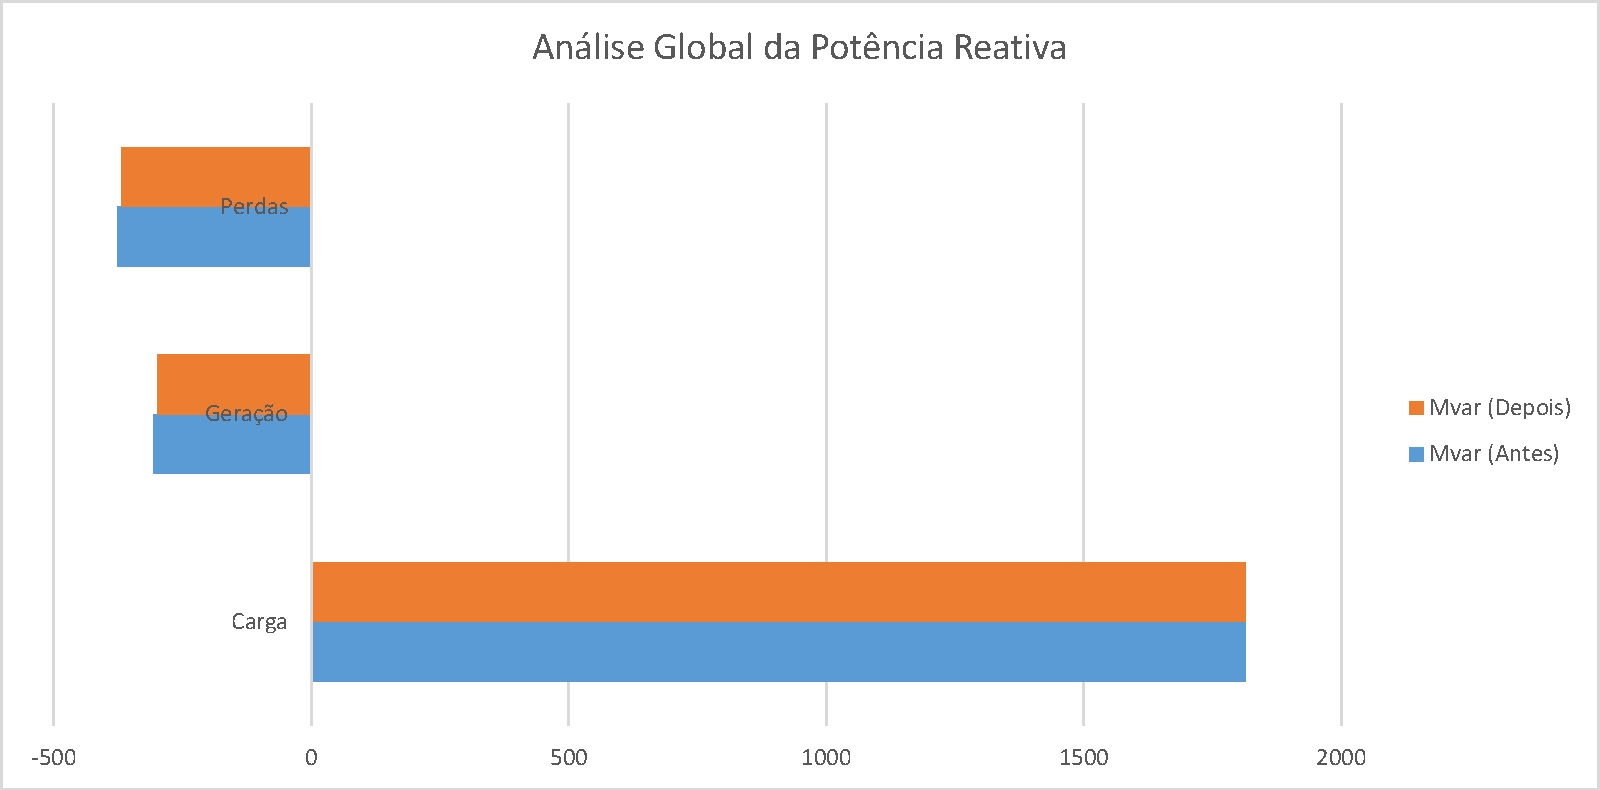
\includegraphics[width=\linewidth]{img/global_MVAr_caso1.pdf}
	\caption{Análise reativa global antes e após o cenário 1}
	\vspace{-3.5mm}
	\caption*{Fonte: autoria própria}
	\label{fig:global_MVAr_caso1}
\end{figure}
\subsubsection{Analisar geradores}

\begin{figure}[H]
	\centering
	\captionsetup{width=\textwidth, font=footnotesize, textfont=bf}	
	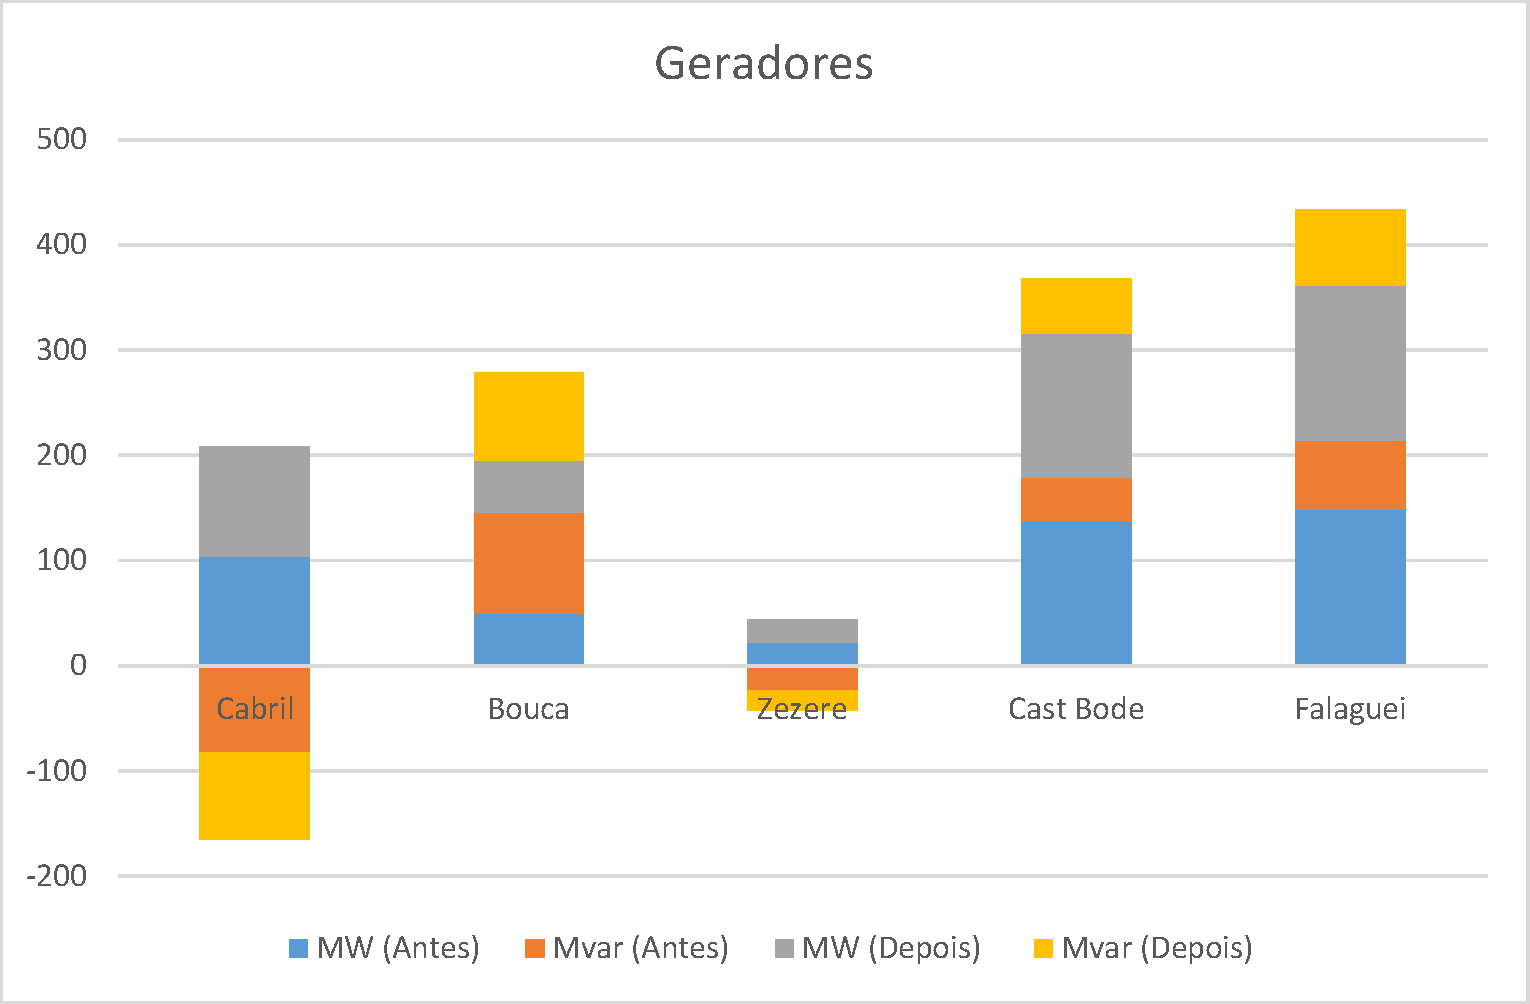
\includegraphics[width=\linewidth]{img/geradores_caso1.pdf}
	\caption{Análise dos geradores antes e após o cenário 1}
	\vspace{-3.5mm}
	\caption*{Fonte: autoria própria}
	\label{fig:geradores_caso1}
\end{figure}


\subsubsection{Análise das linhas}

\begin{figure}[H]
	\centering
	\captionsetup{width=\textwidth, font=footnotesize, textfont=bf}	
	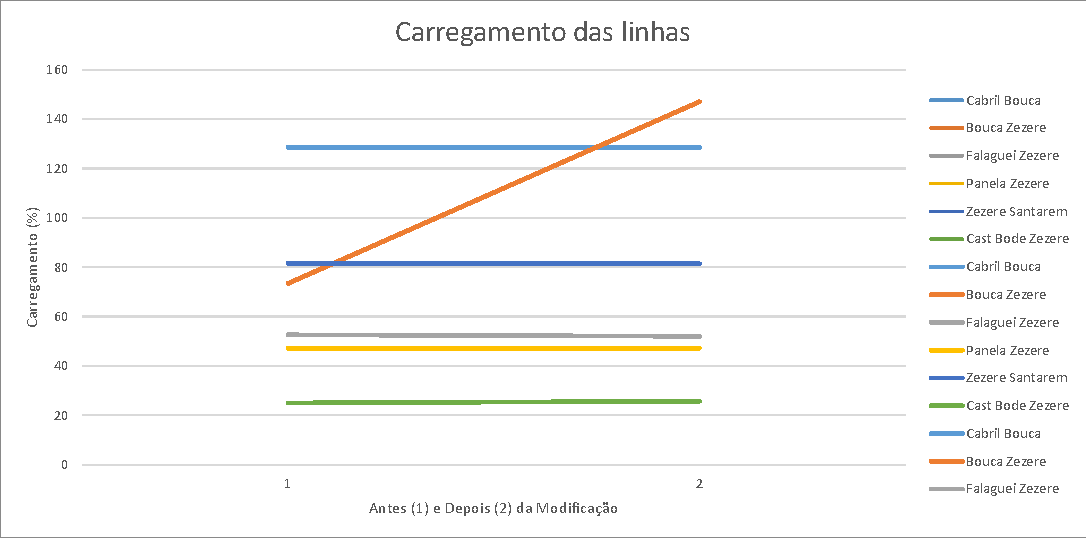
\includegraphics[width=0.9\linewidth]{img/carregamento_linhas_caso1.pdf}
	\caption{Análise do carregamento das linhas antes e após o cenário 1}
	\vspace{-3.5mm}
	\caption*{Fonte: autoria própria}
	\label{fig:carregamento_linhas_caso1}
\end{figure}

	% Mudança do trânsito de potência
	% Sobrecargas
    
\subsubsection{Análise dos barramentos}

\begin{figure}[H]
	\centering
	\captionsetup{width=\textwidth, font=footnotesize, textfont=bf}	
	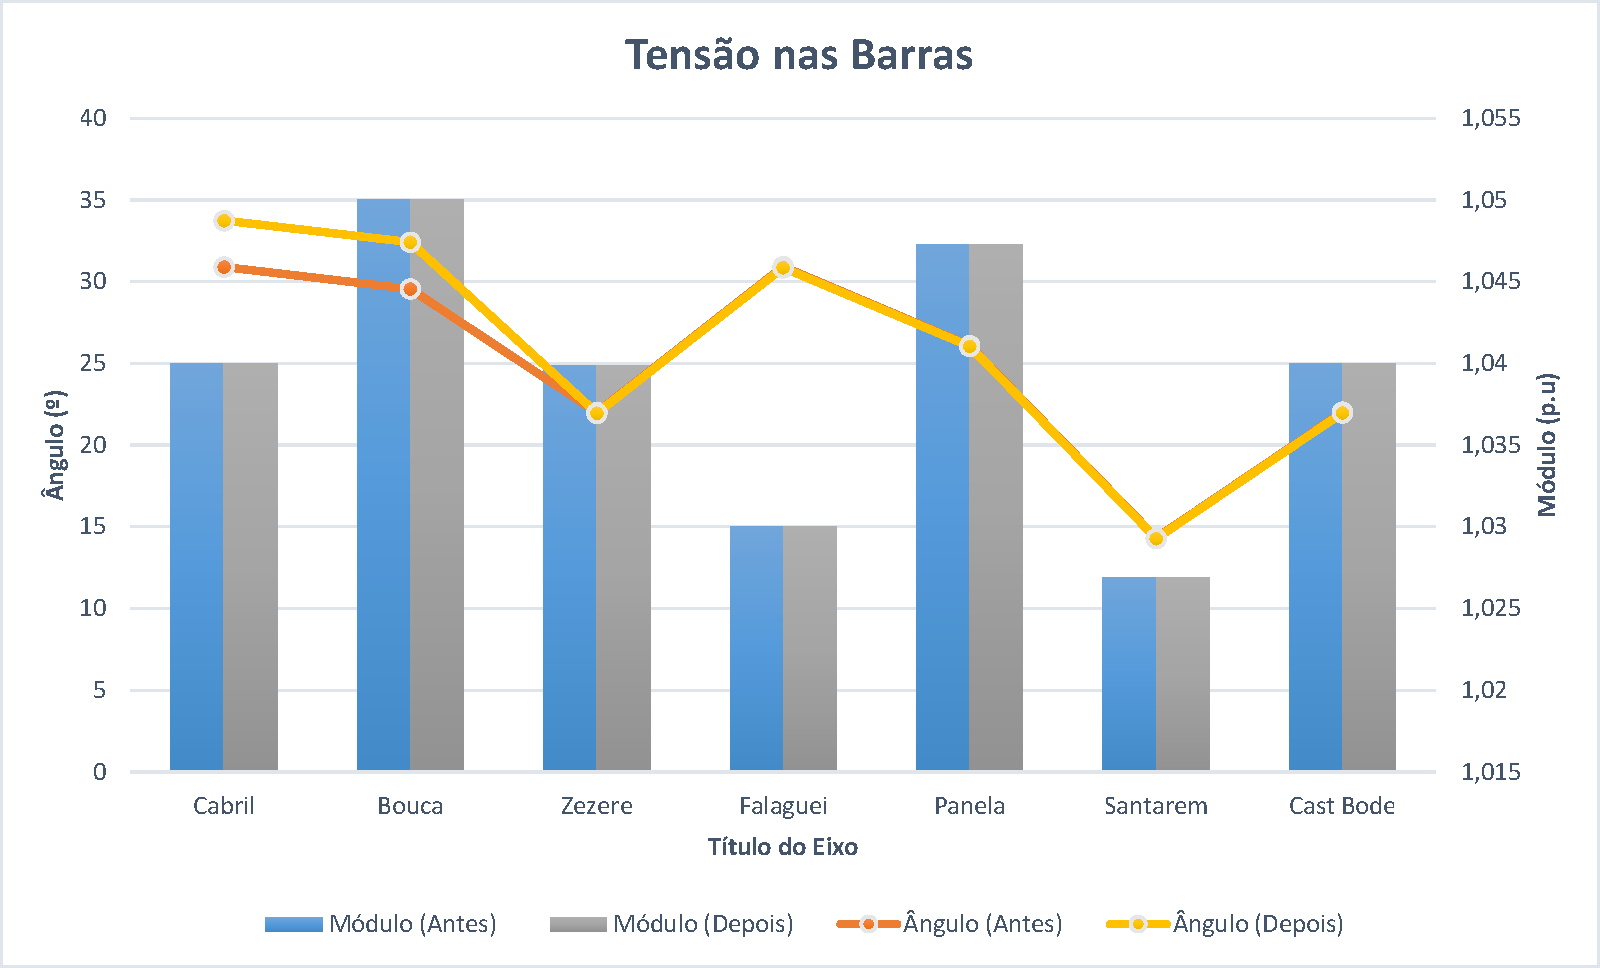
\includegraphics[width=\linewidth]{img/tensoes_barras_caso1.pdf}
	\caption{Análise dos Barramentos Antes e Após o Cenário 1}
	\vspace{-3.5mm}
	\caption*{Fonte: autoria própria}
	\label{fig:tensoes_barras_caso1}
\end{figure}
	% Tensões 
	% Ângulos
    
% ---------- CENÁRIO 2----------
\section{Cenário 2} % Victor
	\subsection{Anterior à modificação}

O cenário 2 escolhido foi na subestação de Pocinho, à margem do Rio Douro, noroeste de Portugal, retratado na Figura \ref{fig:caso_2_antes_geral_menor}. O cenário será a retirada da linha que liga o gerador de Pocinho à subestação de Pocinho, que atualmente está funcionando com 102\% da sua capacidade de trânsito de potência.

\begin{figure}[H]
	\centering
	\captionsetup{width=\textwidth, font=footnotesize, textfont=bf}	
	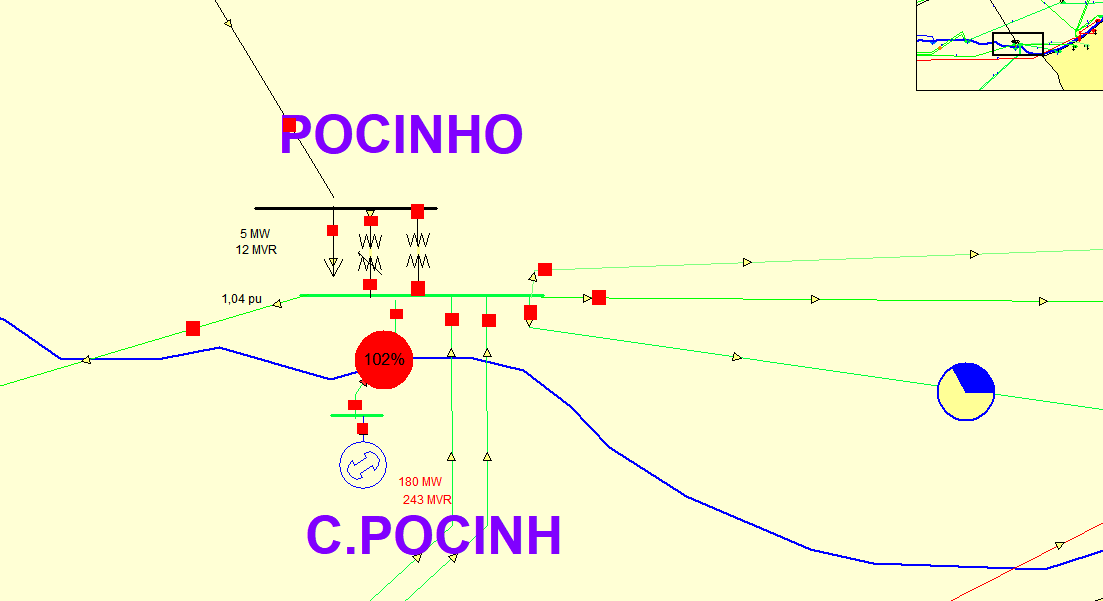
\includegraphics[width=\linewidth]{img/caso_2_antes_geral.PNG}
	\caption{Cenário 2, anterior à modificação}
	\vspace{-3.5mm}
	\caption*{Fonte: autoria própria}
	\label{fig:caso_2_antes_geral_menor}
\end{figure}

Os barramentos que estão diretamente ligados ao barramento (subestação) de Pocinho, circulada em vermelho na Figura \ref{fig:caso_2_antes_geral}, são: M. Cavale, Armamar, Chafariz, Saucelle (Espanha), 489 (Espanha) e Aldeadav (Espanha); todas estas subestações ligadas a Pocinho estão circuladas em azul na Figura \ref{fig:caso_2_antes_geral}.

\begin{figure}[H]
	\centering
	\captionsetup{width=\textwidth, font=footnotesize, textfont=bf}	
	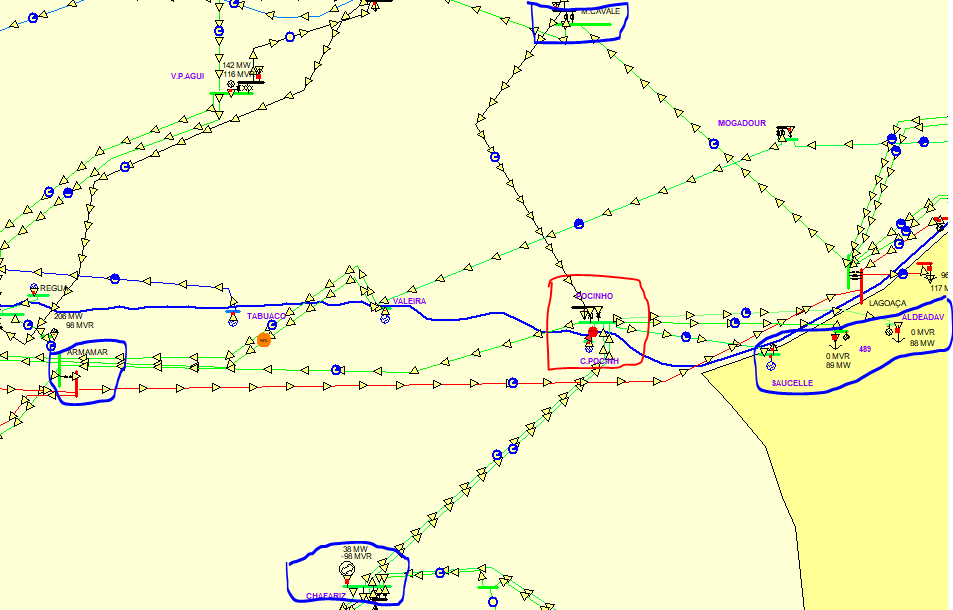
\includegraphics[width=\linewidth]{img/caso_2_antes_expandido.PNG}
	\caption{Vista ampliada do cenário 2, anterior à modificação}
	\vspace{-3.5mm}
	\caption*{Fonte: autoria própria}
	\label{fig:caso_2_antes_geral}
\end{figure}

Os dados globais antes da modificação são os mesmos do caso 1, como pode ser visto na Tabela \ref{tab:DadosGeraisIniciais}. Na Tabela \ref{tab:caso_2_antes} são descritos os valores de geração de potência ativa e reativa do gerador de Pocinho, carregamento das linhas em conexão com a subestação de Pocinho, módulo e ângulo dos barramentos ligados a Pocinho, potência ativa e reativa líquida entre Portugal e Espanha na região próxima a Pocinho, bem como o sentido do fluxo de potência nas linhas.

\begin{table}[H]
\centering
\small
\captionsetup{width=.76\textwidth, font=footnotesize, textfont=bf}
\begin{tabular}{llcc}
\multicolumn{4}{c}{\cellcolor[HTML]{333333}{\color[HTML]{FFFFFF} \textbf{Carregamento das linhas}}} \\
 & \multicolumn{1}{c}{\textbf{Sentido da Potência}} &  & \textbf{Carregamento (\%)} \\
\textbf{Pocinho} & \multicolumn{1}{c}{$<-$} & \multicolumn{1}{l}{\textbf{M. Cavale}} & 2 \\
\textbf{Pocinho} & \multicolumn{1}{c}{$->$} & \multicolumn{1}{l}{\textbf{Armamar}} & 17,3 \\
\textbf{Pocinho} & \multicolumn{1}{c}{$<-$} & \multicolumn{1}{l}{\textbf{Chafariz}} & 6 \\
\textbf{Pocinho} & \multicolumn{1}{c}{$->$} & \multicolumn{1}{l}{\textbf{Saucelle}} & 32,9 \\
\textbf{Pocinho} & \multicolumn{1}{c}{$->$} & \multicolumn{1}{l}{\textbf{489}} & 29,6 \\
\textbf{Pocinho} & \multicolumn{1}{c}{$->$} & \multicolumn{1}{l}{\textbf{Aldedav}} & 29,2 \\
\multicolumn{4}{c}{\cellcolor[HTML]{333333}{\color[HTML]{FFFFFF} \textbf{Tensão nas barras}}} \\
 &  & \textbf{Módulo} & \textbf{Ângulo} \\
\cellcolor[HTML]{036400}{\color[HTML]{FFFFFF} } & \textbf{Pocinho} & 1,0376 & 32,275 \\
\cellcolor[HTML]{036400}{\color[HTML]{FFFFFF} } & \textbf{M. Cavale} & 1,0493 & 33,348 \\
\cellcolor[HTML]{036400}{\color[HTML]{FFFFFF} } & \textbf{Armamar} & 1,0484 & 28,552 \\
\multirow{-4}{*}{\cellcolor[HTML]{036400}{\color[HTML]{FFFFFF} \textbf{Portugal}}} & \textbf{Chafariz} & 1,04 & 32,932 \\
\multicolumn{1}{c}{\cellcolor[HTML]{CD9934}{\color[HTML]{FFFFFF} \textbf{}}} & \textbf{Saucelle} & 1 & 32,206 \\
\cellcolor[HTML]{CD9934}{\color[HTML]{FFFFFF} \textbf{Espannha}} & \textbf{489} & 1 & 30,837 \\
\cellcolor[HTML]{CD9934}{\color[HTML]{FFFFFF} } & \textbf{Aldeadav} & 1 & 30,832 \\
\multicolumn{4}{c}{\cellcolor[HTML]{333333}{\color[HTML]{FFFFFF} \textbf{Geradores}}} \\
 &  & \textbf{MW} & \textbf{MVar} \\
\multicolumn{1}{c}{\cellcolor[HTML]{036400}{\color[HTML]{FFFFFF} }} & \textbf{Pocinho} & 180 & 243 \\
\multicolumn{1}{c}{\multirow{-2}{*}{\cellcolor[HTML]{036400}{\color[HTML]{FFFFFF} \textbf{Portugal}}}} & \textbf{Chafariz} & 38 & -98 \\
\cellcolor[HTML]{CD9934}{\color[HTML]{FFFFFF} } & \textbf{Saucelle} & 0 & -137 \\
\cellcolor[HTML]{CD9934}{\color[HTML]{FFFFFF} \textbf{Espannha}} & \textbf{489} & 0 & -92 \\
\cellcolor[HTML]{CD9934}{\color[HTML]{FFFFFF} } & \textbf{Aldeadav} & 0 & -91 \\
\multicolumn{4}{c}{\cellcolor[HTML]{333333}{\color[HTML]{FFFFFF} \textbf{Interligação com Espanha}}} \\
\multicolumn{2}{l}{\textbf{Portugal $->$ Espanha}} & 208,9 MW & 320,5 MVAr\\
\hline
\end{tabular}
  \caption{Dados iniciais para o caso 2}
  \vspace{-3.5mm}
	\caption*{Fonte: Autoria Própria}
  \label{tab:caso_2_antes}
\end{table}

% - sUBSECTION
\subsection{Análise do impacto da modificação}
Realizando a modificação, abertura da linha que liga o gerador de Pocinho à subestação de Pocinho, conforme a Figura \ref{fig:caso_2_depois_geral_menor} e com vista ampliado na Figura \ref{fig:caso_2_depois_geral}. Na Tabela \ref{tab:caso_2_depois} são descritos os valores para análise após a modificação do caso 2.

\begin{figure}[H]
	\centering
	\captionsetup{width=\textwidth, font=footnotesize, textfont=bf}	
	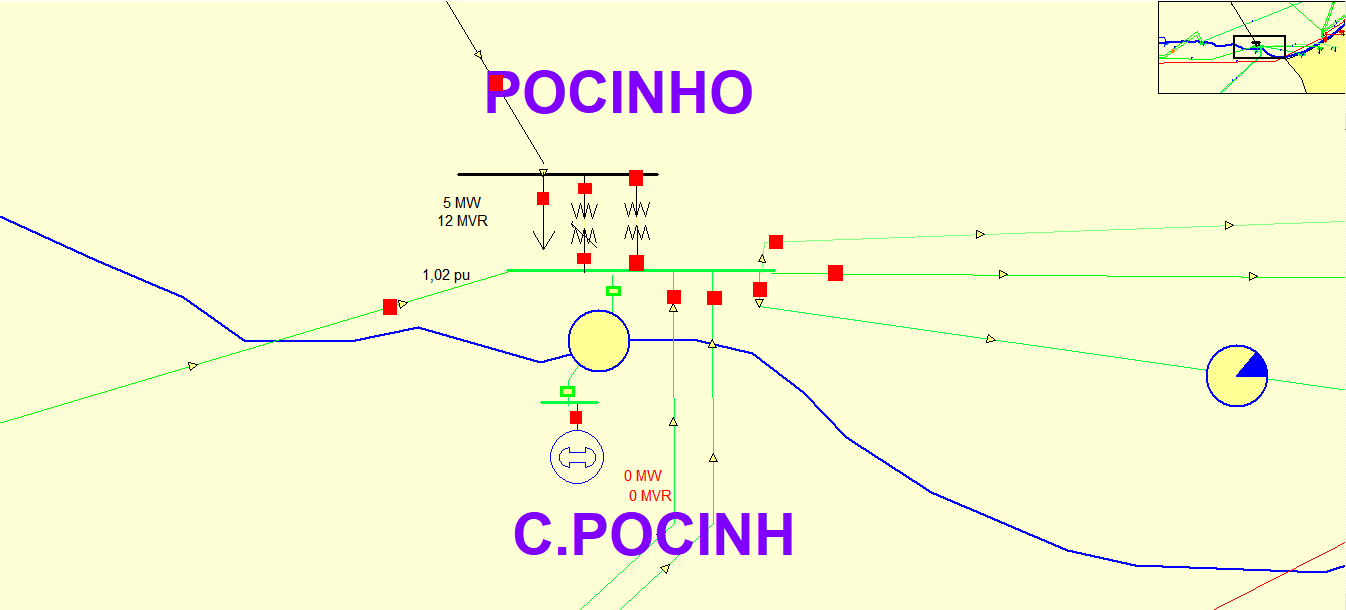
\includegraphics[width=\linewidth]{img/caso_2_depois_geral.PNG}
	\caption{Cenário 2, após a modificação}
	\vspace{-3.5mm}
	\caption*{Fonte: autoria própria}
	\label{fig:caso_2_depois_geral_menor}
\end{figure}

\begin{figure}[H]
	\centering
	\captionsetup{width=\textwidth, font=footnotesize, textfont=bf}	
	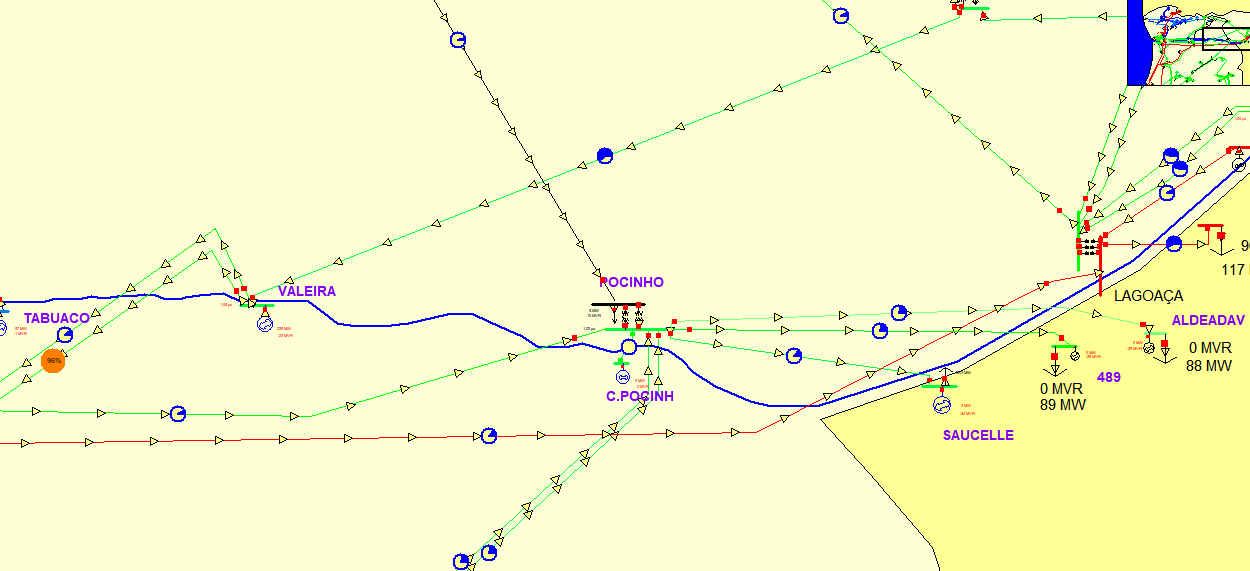
\includegraphics[width=\linewidth]{img/caso_2_depois_expandido.PNG}
	\caption{Vista ampliada do cenário 2, após a modificação}
	\vspace{-3.5mm}
	\caption*{Fonte: autoria própria}
	\label{fig:caso_2_depois_geral}
\end{figure}

\begin{table}[H]
\centering
\small
\captionsetup{width=.76\textwidth, font=footnotesize, textfont=bf}
\begin{tabular}{llcc}
\multicolumn{4}{c}{\cellcolor[HTML]{333333}{\color[HTML]{FFFFFF} \textbf{Carregamento das linhas}}} \\
 & \multicolumn{1}{c}{\textbf{Sentido da Potência}} &  & \textbf{Carregamento (\%)} \\
\textbf{Pocinho} & \multicolumn{1}{c}{$<-$} & \multicolumn{1}{l}{\textbf{M. Cavale}} & 4,3 \\
\textbf{Pocinho} & \multicolumn{1}{c}{$<-$} & \multicolumn{1}{l}{\textbf{Armamar}} & 9 \\
\textbf{Pocinho} & \multicolumn{1}{c}{$<-$} & \multicolumn{1}{l}{\textbf{Chafariz}} & 21,8 \\
\textbf{Pocinho} & \multicolumn{1}{c}{$->$} & \multicolumn{1}{l}{\textbf{Saucelle}} & 13,8 \\
\textbf{Pocinho} & \multicolumn{1}{c}{$->$} & \multicolumn{1}{l}{\textbf{489}} & 21,5 \\
\textbf{Pocinho} & \multicolumn{1}{c}{$->$} & \multicolumn{1}{l}{\textbf{Aldedav}} & 21,2 \\
\multicolumn{4}{c}{\cellcolor[HTML]{333333}{\color[HTML]{FFFFFF} \textbf{Tensão nas barras}}} \\
 &  & \textbf{Módulo} & \textbf{Ângulo} \\
\cellcolor[HTML]{036400}{\color[HTML]{FFFFFF} } & \textbf{Pocinho} & 1,0155 & 25,644 \\
\cellcolor[HTML]{036400}{\color[HTML]{FFFFFF} } & \textbf{M. Cavale} & 1,0384 & 28,661 \\
\cellcolor[HTML]{036400}{\color[HTML]{FFFFFF} } & \textbf{Armamar} & 1,0498 & 25,102 \\
\multirow{-4}{*}{\cellcolor[HTML]{036400}{\color[HTML]{FFFFFF} \textbf{Portugal}}} & \textbf{Chafariz} & 1,0400 & 27,690 \\
\multicolumn{1}{c}{\cellcolor[HTML]{CD9934}{\color[HTML]{FFFFFF} \textbf{}}} & \textbf{Saucelle} & 1 & 25,349 \\
\cellcolor[HTML]{CD9934}{\color[HTML]{FFFFFF} \textbf{Espannha}} & \textbf{489} & 1 & 23,953 \\
\cellcolor[HTML]{CD9934}{\color[HTML]{FFFFFF} } & \textbf{Aldeadav} & 1 & 23,950 \\
\multicolumn{4}{c}{\cellcolor[HTML]{333333}{\color[HTML]{FFFFFF} \textbf{Geradores}}} \\
 &  & \textbf{MW} & \textbf{MVar} \\
\multicolumn{1}{c}{\cellcolor[HTML]{036400}{\color[HTML]{FFFFFF} }} & \textbf{Pocinho} & 0 & 0 \\
\multicolumn{1}{c}{\multirow{-2}{*}{\cellcolor[HTML]{036400}{\color[HTML]{FFFFFF} \textbf{Portugal}}}} & \textbf{Chafariz} & 38 & -18 \\
\cellcolor[HTML]{CD9934}{\color[HTML]{FFFFFF} } & \textbf{Saucelle} & 0 & -54 \\
\cellcolor[HTML]{CD9934}{\color[HTML]{FFFFFF} \textbf{Espannha}} & \textbf{489} & 0 & -29 \\
\cellcolor[HTML]{CD9934}{\color[HTML]{FFFFFF} } & \textbf{Aldeadav} & 0 & -29 \\
\multicolumn{4}{c}{\cellcolor[HTML]{333333}{\color[HTML]{FFFFFF} \textbf{Interligação com Espanha}}} \\
\multicolumn{2}{l}{\textbf{Portugal $->$ Espanha}} & 207,2 MW & 104,8 MVAr\\
\hline
\end{tabular}
  \caption{Dados após modificação para o caso 2}
  \vspace{-3.5mm}
	\caption*{Fonte: Autoria Própria}
  \label{tab:caso_2_depois}
\end{table}

Inicialmente é possível verificar que a linha entre Pocinho e Armamar alterou o sentido do fluxo de potência. Isso pode ser explicado pelo facto que o gerador de Pocinho estava a enviar potência para a interligação com a Espanha e ainda alimentava Armamar; com a sua retirada, houve necessidade de alimentar a interligação com a Espanha com potência ativa de outros geradores, como as outras linhas em contacto com Pocinho já estavam no sentido de enviar potência para ela, ficou apenas a linha com Armamar a alterar o sentido. Os dados globais do sistema após a modificação estão mostrados na Tabela \ref{tab:DadosGerais_caso_2}. A seguir irá ser analisado com mais detalhes os impactos do caso em estudo.

\begin{table}[H]
\centering
	\captionsetup{width=0.4\textwidth, font=footnotesize, textfont=bf}
    \begin{tabular}{|
  >{\columncolor[HTML]{000000}}l |c|c|l}
  \cline{1-3}
  {\color[HTML]{FFFFFF} } & \cellcolor[HTML]{000000}{\color[HTML]{FFFFFF} MW} & \cellcolor[HTML]{000000}{\color[HTML]{FFFFFF} MVAr} &  \\ \cline{1-3}
  {\color[HTML]{FFFFFF} Perdas}  & 207,58 & -568,00  &  \\ \cline{1-3}
  {\color[HTML]{FFFFFF} Geração} & 6772,1 & -504,4  &  \\ \cline{1-3}
  {\color[HTML]{FFFFFF} Cargas}  & 6564,5 & 1814,2 &  \\ \cline{1-3}
  \end{tabular}
  \caption{Dados gerais após caso 2}
  \vspace{-3.5mm}
	\caption*{Fonte: Autoria Própria}
  \label{tab:DadosGerais_caso_2}
\end{table}

\subsubsection{Análise global}
Os impactos da modificação na análise global estão resumidos no gráfico da Figura \ref{fig:global_MW_caso2} para a potência ativa e na Figura \ref{fig:global_MVAr_caso2} para a potência reativa.

\begin{figure}[H]
	\centering
	\captionsetup{width=\textwidth, font=footnotesize, textfont=bf}	
	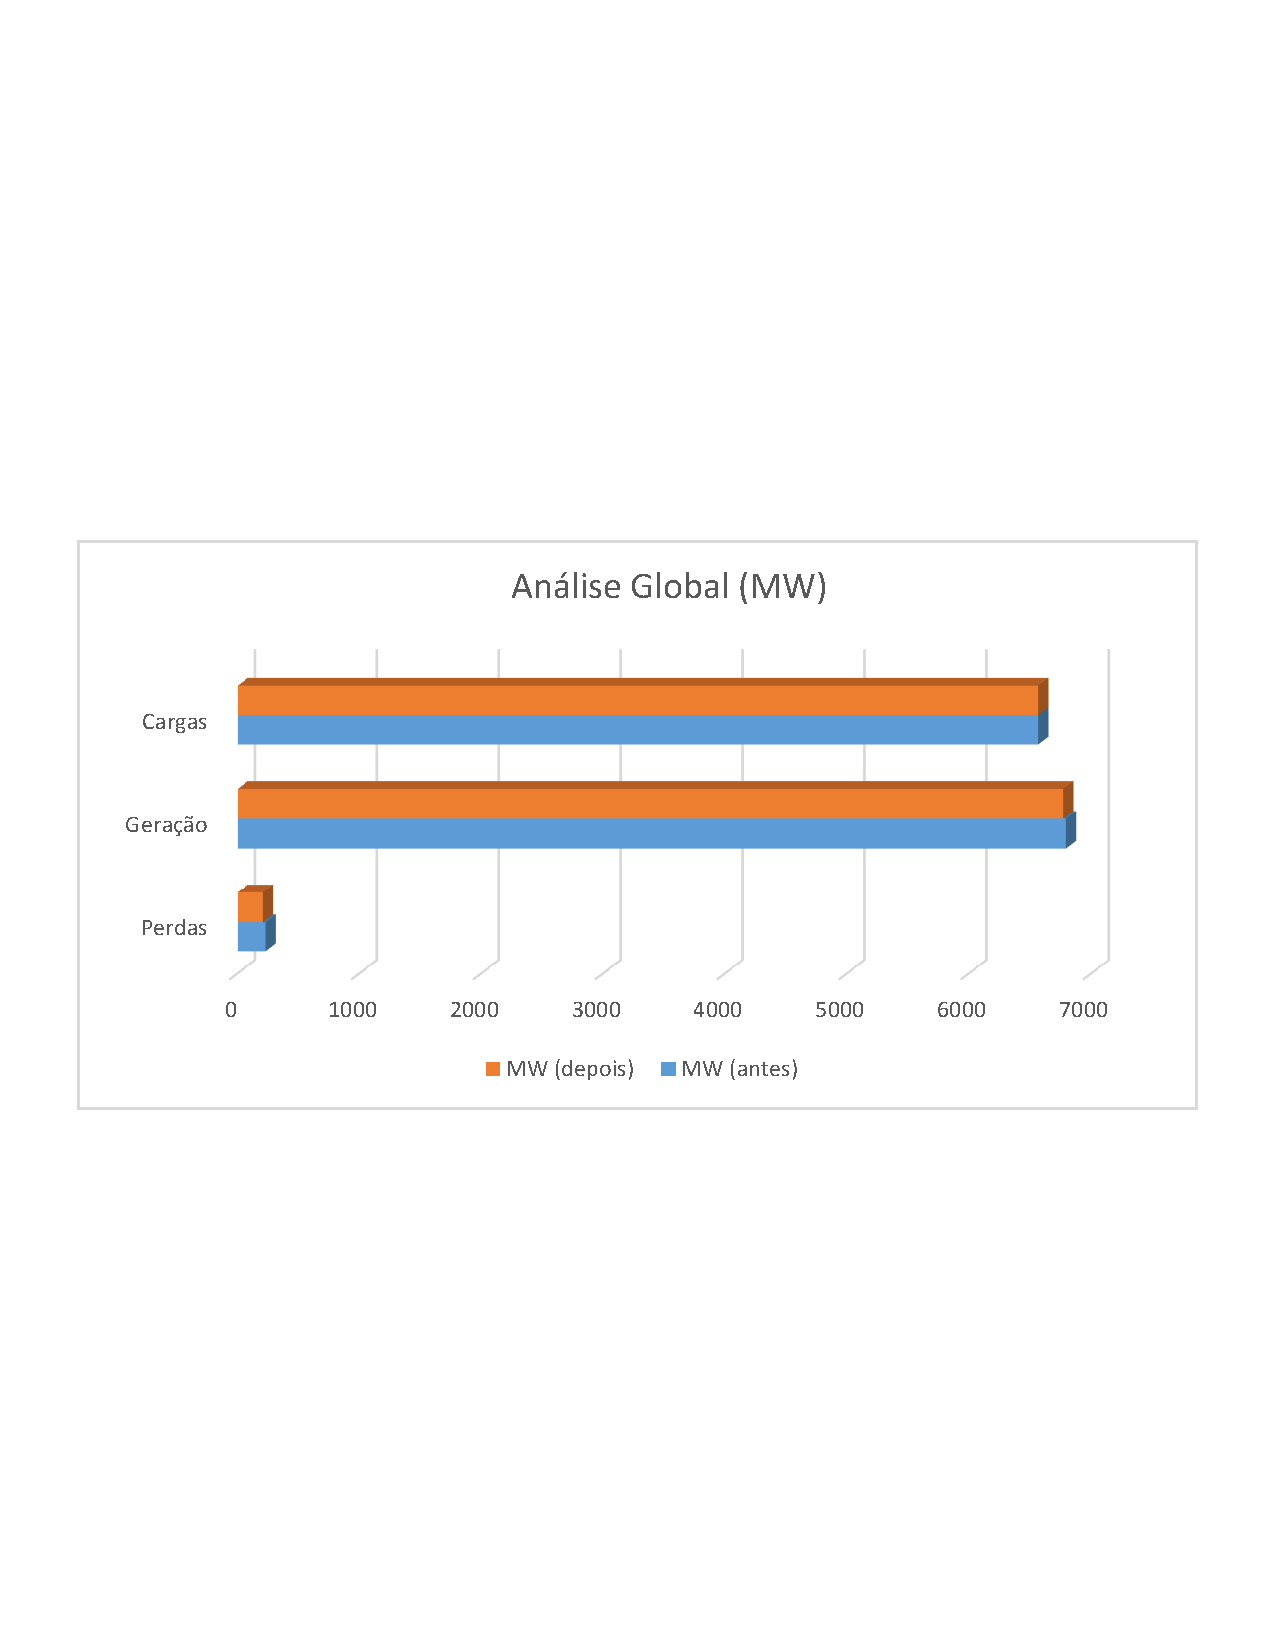
\includegraphics[width=\linewidth,trim = 20mm 97mm 20mm 105mm,clip]{img/global_MW_caso2.pdf}
	\caption{Análise ativa global antes e após o cenário 2}
	\vspace{-3.5mm}
	\caption*{Fonte: autoria própria}
	\label{fig:global_MW_caso2}
\end{figure}

Pelas Figuras \ref{fig:global_MW_caso2} e \ref{fig:global_MVAr_caso2} é atestado que as cargas não variaram, o que mostra que apenas foi retirado geração. Um facto interessante é que as perdas ativas globais diminuíram, isso pode ser explicado porque as linhas que aumentaram o carregamento foram as linhas Pocinho - Chafariz e Pocinho - M. Cavale, sendo que a Pocinho - Chafariz passou de 6\% para 21,8\% de carregamento, conforme Figura \ref{fig:carregamento_linhas_caso2}. 

\begin{figure}[H]
	\centering
	\captionsetup{width=\textwidth, font=footnotesize, textfont=bf}	
	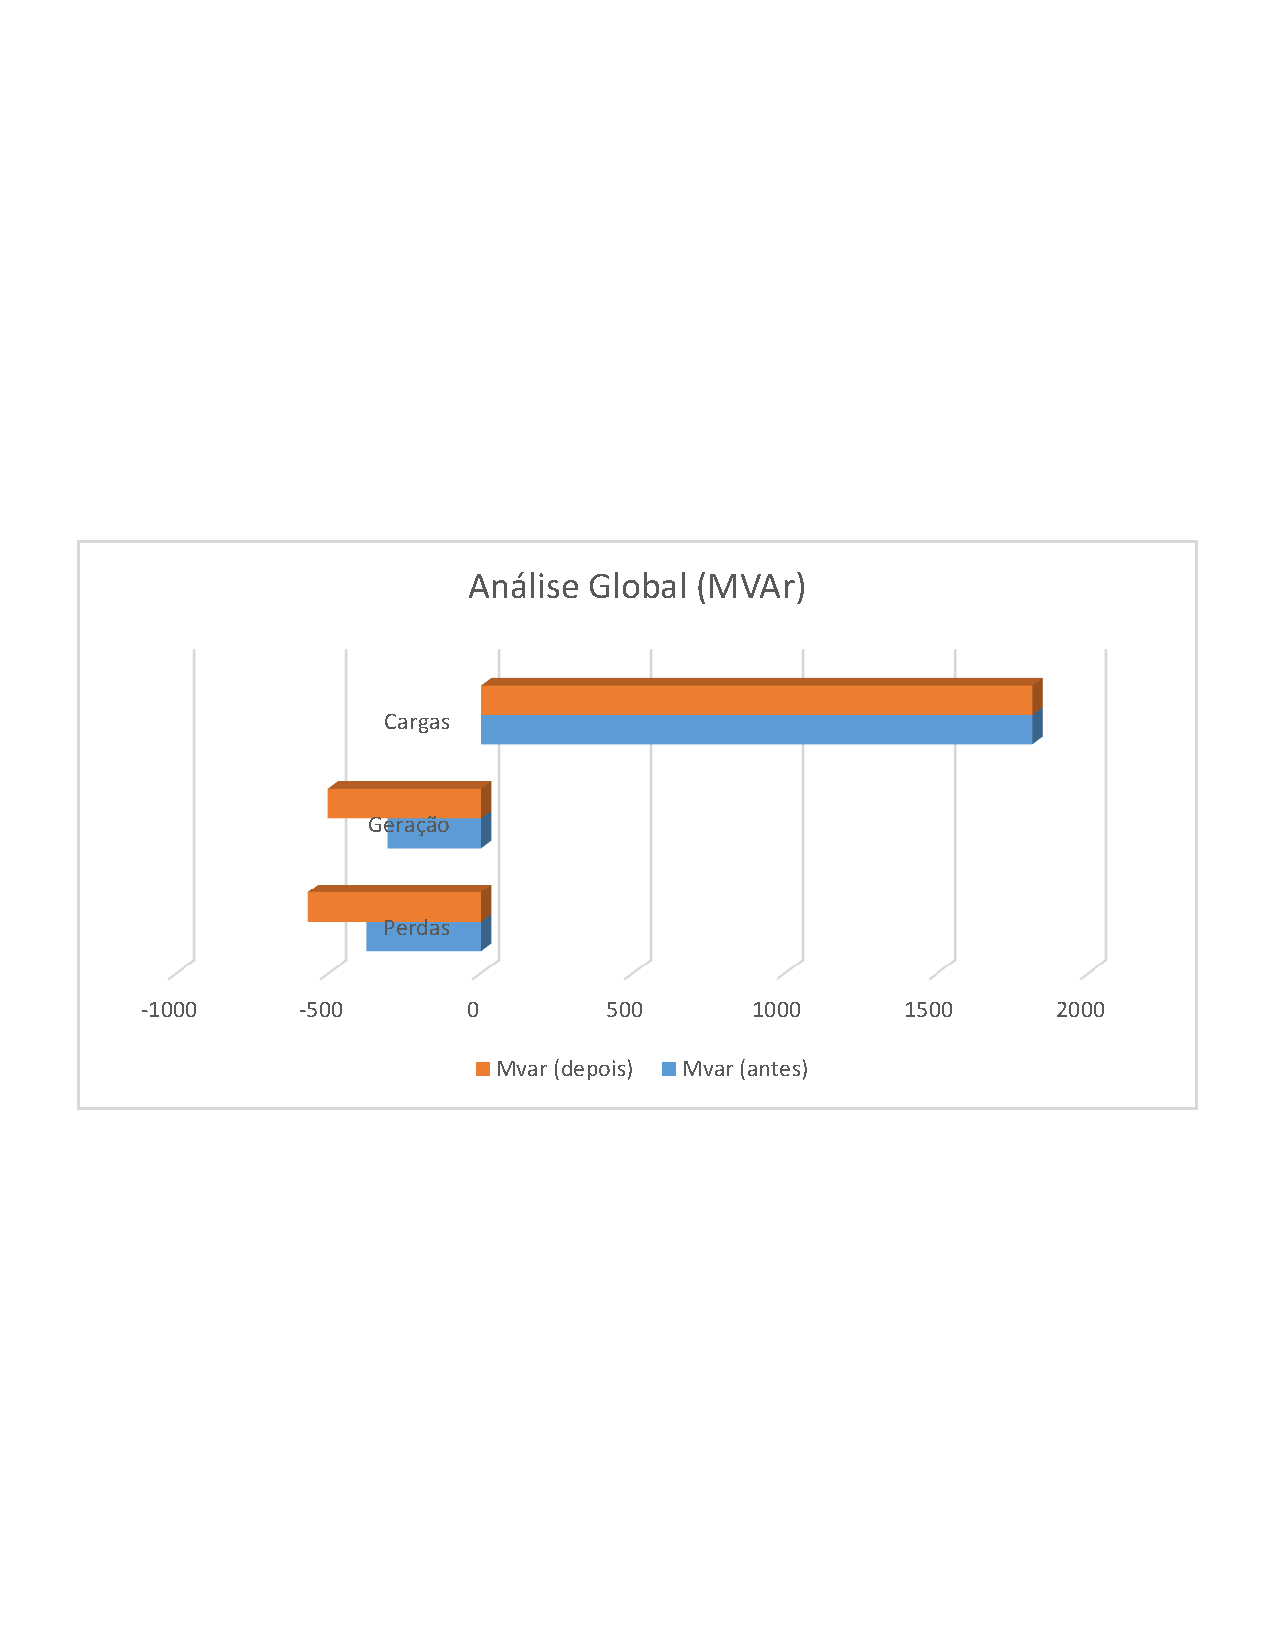
\includegraphics[width=\linewidth,trim = 20mm 97mm 20mm 105mm,clip]{img/global_MVAr_caso2.pdf}
	\caption{Análise reativa global antes e após o cenário 2}
	\vspace{-3.5mm}
	\caption*{Fonte: autoria própria}
	\label{fig:global_MVAr_caso2}
\end{figure}

Observando o gráfico da Figura \ref{fig:global_MVAr_caso2} é visto que houve maior produção de potência reativa capacitiva a fim de atender a também elevação das potência reativa capacitiva das perdas, estas devido ao aumento de carregamento das linhas, o que ocasiona maior efeito capacitivo nas linhas de transmissão.

\subsubsection{Analisar geradores}
O impacto da modificação nos geradores dos barramentos próximos estão resumidas no gráfico da Figura \ref{fig:geradores_caso2}. É evidente a saída da contribuição do gerador de Pocinho, outro facto evidente é a redução da geração de potência reativa capacitiva neste grupo de geradores. Tal redução de capacitivo pode ser explicado pelo fato que antes o gerador de Pocinho gerava apenas potência reativa indutiva, com a saída dele, os outros geradores tiveram que gerar menos capacitivo. 

\begin{figure}[H]
	\centering
	\captionsetup{width=\textwidth, font=footnotesize, textfont=bf}	
	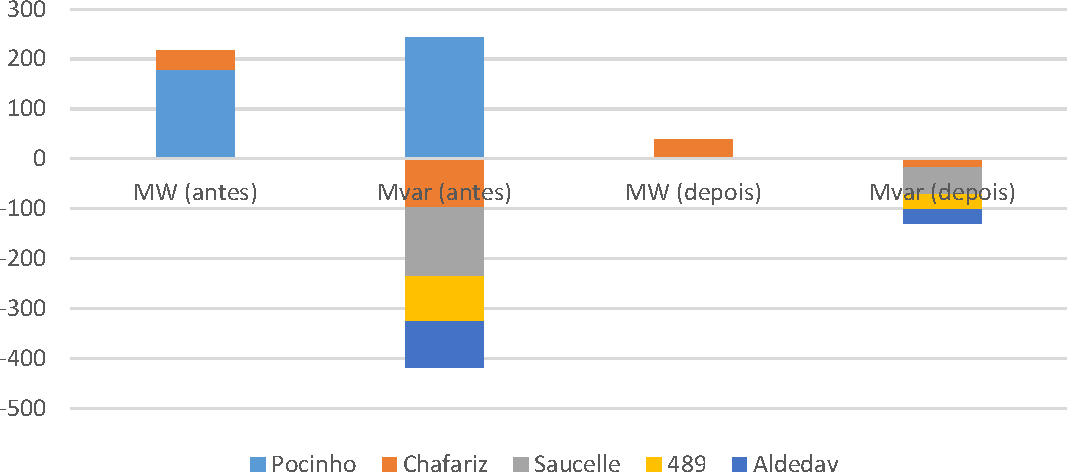
\includegraphics[width=\linewidth]{img/geradores_caso2.pdf}
	\caption{Análise dos geradores antes e após o cenário 2}
	\vspace{-3.5mm}
	\caption*{Fonte: autoria própria}
	\label{fig:geradores_caso2}
\end{figure}

\subsubsection{Análise das linhas}
Os impactos da modificação no carregamento das linhas ligadas à subestação de Pocinho estão resumidos no gráfico da Figura \ref{fig:carregamento_linhas_caso2}.

\begin{figure}[H]
	\centering
	\captionsetup{width=\textwidth, font=footnotesize, textfont=bf}	
	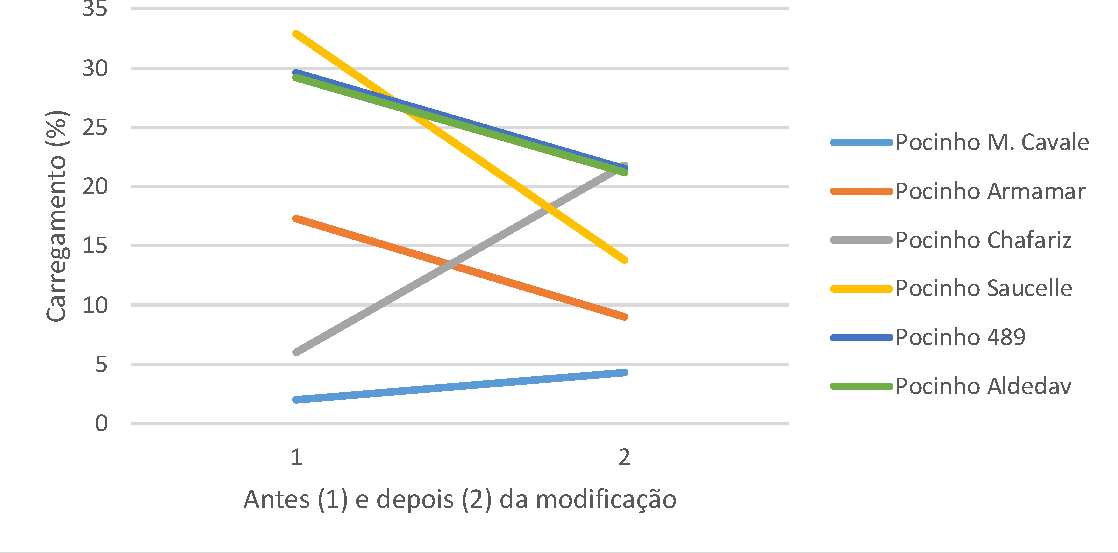
\includegraphics[width=\linewidth]{img/carregamento_linhas_caso2.pdf}
	\caption{Análise do carregamento das linhas antes e após o cenário 2}
	\vspace{-3.5mm}
	\caption*{Fonte: autoria própria}
	\label{fig:carregamento_linhas_caso2}
\end{figure}

Em resumo, as linhas de Pocinha a Saucelle, Armamar, 489, e Aldedav foram as que tiveram redução no carregamento, isso decorre do fato que estas linhas eram as que estavam levando parte da potência gerada pelo gerador de Pocinho, como ele foi tirado de operação, não há mais essa potência a passar por essas linhas. A justificativa oposta se aplica à elevação do carregamento apenas nas linhas entre Pocinho a Chafariz, e M. Cavale, haja vista que essas linhas eram as únicas que inicialmente mandavam potência para Pocinho. O sentido do fluxo de potência na linha entre Pocinho e Armamar mudou devido a necessidade de suprir a carga antes atendida pelo gerador de Pocinho.

% comentar
\subsubsection{Análise dos barramentos}
Os impactos da modificação nos barramentos ligados à subestação de Pocinho estão resumidos no gráfico da Figura \ref{fig:tensoes_barras_caso2}.

\begin{figure}[H]
	\centering
	\captionsetup{width=\textwidth, font=footnotesize, textfont=bf}	
	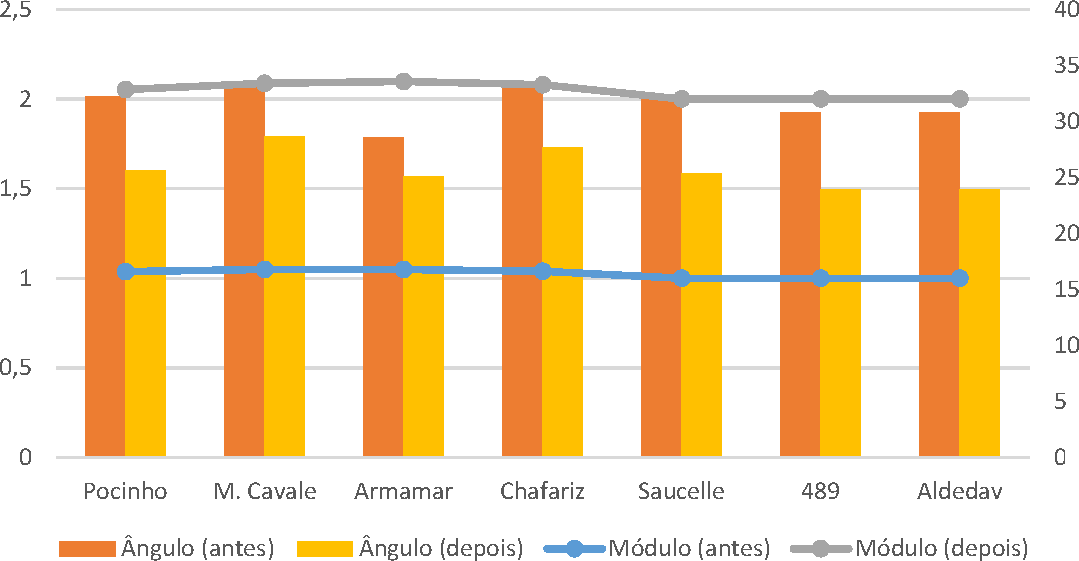
\includegraphics[width=\linewidth]{img/tensoes_barras_caso2.pdf}
	\caption{Análise dos barramentos antes e após o cenário 2}
	\vspace{-3.5mm}
	\caption*{Fonte: autoria própria}
	\label{fig:tensoes_barras_caso2}
\end{figure}

% comentar
\subsubsection{Análise da interligação com a Espanha}
Os impactos da modificação na interligação com a Espanha estão resumidos na Tabela \ref{tab:espanha_caso2}.

\begin{table}[H]
\centering
	\captionsetup{width=0.4\textwidth, font=footnotesize, textfont=bf}
    \begin{tabular}{|
  >{\columncolor[HTML]{000000}}l |c|c|l}
  \cline{1-3}
  {\color[HTML]{FFFFFF} } & \cellcolor[HTML]{000000}{\color[HTML]{FFFFFF} MW} & \cellcolor[HTML]{000000}{\color[HTML]{FFFFFF} MVAr} &  \\ \cline{1-3}
  {\color[HTML]{FFFFFF} Antes}  & 208,9 & 320,5 &  \\ \cline{1-3}
  {\color[HTML]{FFFFFF} Depois} & 207,2 & 104,8 &  \\ \cline{1-3}
  \end{tabular}
  \caption{Interligação com a Espanha antes e após o cenário 2}
  \vspace{-3.5mm}
	\caption*{Fonte: Autoria Própria}
  \label{tab:espanha_caso2}
\end{table}


%\chapter{Critérios de análise e validação das soluções} 
%\input{src/Criterios_analise.tex}

%\chapter{Simulação} 
%\input{src/Simulacao.tex}

%\chapter{Análise crítica} 
%\input{src/Analise_critica.tex}

\chapter{Conclusão} 
\input{src/Conclusao.tex}

%% Bibliografia
\bibliography{bibliografia}

\end{document}